\documentclass[twoside]{book}

% Packages required by doxygen
\usepackage{fixltx2e}
\usepackage{calc}
\usepackage{doxygen}
\usepackage[export]{adjustbox} % also loads graphicx
\usepackage{graphicx}
\usepackage[utf8]{inputenc}
\usepackage{makeidx}
\usepackage{multicol}
\usepackage{multirow}
\PassOptionsToPackage{warn}{textcomp}
\usepackage{textcomp}
\usepackage[nointegrals]{wasysym}
\usepackage[table]{xcolor}

% Font selection
\usepackage[T1]{fontenc}
\usepackage[scaled=.90]{helvet}
\usepackage{courier}
\usepackage{amssymb}
\usepackage{sectsty}
\renewcommand{\familydefault}{\sfdefault}
\allsectionsfont{%
  \fontseries{bc}\selectfont%
  \color{darkgray}%
}
\renewcommand{\DoxyLabelFont}{%
  \fontseries{bc}\selectfont%
  \color{darkgray}%
}
\newcommand{\+}{\discretionary{\mbox{\scriptsize$\hookleftarrow$}}{}{}}

% Page & text layout
\usepackage{geometry}
\geometry{%
  a4paper,%
  top=2.5cm,%
  bottom=2.5cm,%
  left=2.5cm,%
  right=2.5cm%
}
\tolerance=750
\hfuzz=15pt
\hbadness=750
\setlength{\emergencystretch}{15pt}
\setlength{\parindent}{0cm}
\setlength{\parskip}{3ex plus 2ex minus 2ex}
\makeatletter
\renewcommand{\paragraph}{%
  \@startsection{paragraph}{4}{0ex}{-1.0ex}{1.0ex}{%
    \normalfont\normalsize\bfseries\SS@parafont%
  }%
}
\renewcommand{\subparagraph}{%
  \@startsection{subparagraph}{5}{0ex}{-1.0ex}{1.0ex}{%
    \normalfont\normalsize\bfseries\SS@subparafont%
  }%
}
\makeatother

% Headers & footers
\usepackage{fancyhdr}
\pagestyle{fancyplain}
\fancyhead[LE]{\fancyplain{}{\bfseries\thepage}}
\fancyhead[CE]{\fancyplain{}{}}
\fancyhead[RE]{\fancyplain{}{\bfseries\leftmark}}
\fancyhead[LO]{\fancyplain{}{\bfseries\rightmark}}
\fancyhead[CO]{\fancyplain{}{}}
\fancyhead[RO]{\fancyplain{}{\bfseries\thepage}}
\fancyfoot[LE]{\fancyplain{}{}}
\fancyfoot[CE]{\fancyplain{}{}}
\fancyfoot[RE]{\fancyplain{}{\bfseries\scriptsize Generated by Doxygen }}
\fancyfoot[LO]{\fancyplain{}{\bfseries\scriptsize Generated by Doxygen }}
\fancyfoot[CO]{\fancyplain{}{}}
\fancyfoot[RO]{\fancyplain{}{}}
\renewcommand{\footrulewidth}{0.4pt}
\renewcommand{\chaptermark}[1]{%
  \markboth{#1}{}%
}
\renewcommand{\sectionmark}[1]{%
  \markright{\thesection\ #1}%
}

% Indices & bibliography
\usepackage{natbib}
\usepackage[titles]{tocloft}
\setcounter{tocdepth}{3}
\setcounter{secnumdepth}{5}
\makeindex

% Hyperlinks (required, but should be loaded last)
\usepackage{ifpdf}
\ifpdf
  \usepackage[pdftex,pagebackref=true]{hyperref}
\else
  \usepackage[ps2pdf,pagebackref=true]{hyperref}
\fi
\hypersetup{%
  colorlinks=true,%
  linkcolor=blue,%
  citecolor=blue,%
  unicode%
}

% Custom commands
\newcommand{\clearemptydoublepage}{%
  \newpage{\pagestyle{empty}\cleardoublepage}%
}

\usepackage{caption}
\captionsetup{labelsep=space,justification=centering,font={bf},singlelinecheck=off,skip=4pt,position=top}

%===== C O N T E N T S =====

\begin{document}

% Titlepage & ToC
\hypersetup{pageanchor=false,
             bookmarksnumbered=true,
             pdfencoding=unicode
            }
\pagenumbering{roman}
\begin{titlepage}
\vspace*{7cm}
\begin{center}%
{\Large Flex Network Architecture \\[1ex]\large 1.\+0.\+0 }\\
\vspace*{1cm}
{\large Generated by Doxygen 1.8.11}\\
\end{center}
\end{titlepage}
\clearemptydoublepage
\tableofcontents
\clearemptydoublepage
\pagenumbering{arabic}
\hypersetup{pageanchor=true}

%--- Begin generated contents ---
\chapter{versatile}
\label{md_README}
\hypertarget{md_README}{}
wireshark\+: the dissector files for the flex ID

resolver\+: resolver code \begin{DoxyVerb}- 2016/resolver_per.py: socketIO version

-     /resolver.py: non socketIO version

- 2017/resolver.py: pub/sub version
\end{DoxyVerb}


compile and install
\begin{DoxyItemize}
\item source code\+: flex-\/1.\+0.\+tar.\+gz tar xvzf flex-\/1.\+0.\+tar.\+gz cd flex-\/1.\+0 make \&\& sudo make install
\item github\+: git clone \href{https://github.com/hw5773/versatile.git}{\tt https\+://github.\+com/hw5773/versatile.\+git} cd versatile make \&\& sudo make uninstall
\end{DoxyItemize}

uninstall and clean
\begin{DoxyItemize}
\item in the source code directory sudo make uninstall \&\& make clean 
\end{DoxyItemize}
\chapter{R\+E\+A\+D\+ME}
\label{md_socket_README}
\hypertarget{md_socket_README}{}
Note that the signature of sendmsg in proto\+\_\+ops in Linux 2.\+6 is different from that in Linux version above 3.\+0

In Linux 2.\+6\+: int ($\ast$sendmsg) (struct socket $\ast$sock, struct msghdr $\ast$m, size\+\_\+t total\+\_\+len); int ($\ast$recvmsg) (struct socket $\ast$sock, struct msghdr $\ast$m, size\+\_\+t total\+\_\+len, int flags);

In Linux above 3\+: int ($\ast$sendmsg) (struct kiocb $\ast$iocb, struct socket $\ast$sock, struct msghdr $\ast$m, size\+\_\+t total\+\_\+len); int ($\ast$recvmsg) (struct kiocb $\ast$iocb, struct socket $\ast$sock, struct msghdr $\ast$m, size\+\_\+t total\+\_\+len, int flags);

Description of Socket operations connect\+:
\begin{DoxyItemize}
\item binds the target id with the socket 
\end{DoxyItemize}
\chapter{Class Index}
\section{Class List}
Here are the classes, structs, unions and interfaces with brief descriptions\+:\begin{DoxyCompactList}
\item\contentsline{section}{\hyperlink{structflex__sock}{flex\+\_\+sock} \\*The data structure for the Flex specified socket }{\pageref{structflex__sock}}{}
\item\contentsline{section}{\hyperlink{structflexhdr}{flexhdr} }{\pageref{structflexhdr}}{}
\item\contentsline{section}{\hyperlink{structflexid}{flexid} }{\pageref{structflexid}}{}
\item\contentsline{section}{\hyperlink{structflexidhdr}{flexidhdr} }{\pageref{structflexidhdr}}{}
\item\contentsline{section}{\hyperlink{structhash__entry}{hash\+\_\+entry} }{\pageref{structhash__entry}}{}
\item\contentsline{section}{\hyperlink{structhash__table}{hash\+\_\+table} }{\pageref{structhash__table}}{}
\item\contentsline{section}{\hyperlink{structid__manage__ops}{id\+\_\+manage\+\_\+ops} }{\pageref{structid__manage__ops}}{}
\item\contentsline{section}{\hyperlink{structlist__head}{list\+\_\+head} }{\pageref{structlist__head}}{}
\item\contentsline{section}{\hyperlink{structquery__list}{query\+\_\+list} }{\pageref{structquery__list}}{}
\item\contentsline{section}{\hyperlink{structreply__list}{reply\+\_\+list} }{\pageref{structreply__list}}{}
\item\contentsline{section}{\hyperlink{structrepo}{repo} }{\pageref{structrepo}}{}
\item\contentsline{section}{\hyperlink{structresponse}{response} }{\pageref{structresponse}}{}
\item\contentsline{section}{\hyperlink{structrflexhdr}{rflexhdr} }{\pageref{structrflexhdr}}{}
\item\contentsline{section}{\hyperlink{structrflexhdr__ext}{rflexhdr\+\_\+ext} }{\pageref{structrflexhdr__ext}}{}
\item\contentsline{section}{\hyperlink{structsockaddr__flex}{sockaddr\+\_\+flex} }{\pageref{structsockaddr__flex}}{}
\item\contentsline{section}{\hyperlink{structu__hslot}{u\+\_\+hslot} }{\pageref{structu__hslot}}{}
\item\contentsline{section}{\hyperlink{structu__table}{u\+\_\+table} }{\pageref{structu__table}}{}
\item\contentsline{section}{\hyperlink{structuflexhdr}{uflexhdr} }{\pageref{structuflexhdr}}{}
\item\contentsline{section}{\hyperlink{structuflexhdr__ext}{uflexhdr\+\_\+ext} }{\pageref{structuflexhdr__ext}}{}
\end{DoxyCompactList}

\chapter{File Index}
\section{File List}
Here is a list of all documented files with brief descriptions\+:\begin{DoxyCompactList}
\item\contentsline{section}{apps/ipv4/{\bfseries proto\+\_\+flex.\+h} }{\pageref{proto__flex_8h}}{}
\item\contentsline{section}{flexid/{\bfseries flex\+\_\+id.\+h} }{\pageref{flexid_2flex__id_8h}}{}
\item\contentsline{section}{include/flex/{\bfseries flex.\+h} }{\pageref{flex_8h}}{}
\item\contentsline{section}{include/flex/{\bfseries flex\+\_\+addr.\+h} }{\pageref{flex__addr_8h}}{}
\item\contentsline{section}{include/flex/{\bfseries flex\+\_\+const.\+h} }{\pageref{flex__const_8h}}{}
\item\contentsline{section}{include/flex/{\bfseries flex\+\_\+err.\+h} }{\pageref{flex__err_8h}}{}
\item\contentsline{section}{include/flex/{\bfseries flex\+\_\+hdr.\+h} }{\pageref{flex__hdr_8h}}{}
\item\contentsline{section}{include/flex/{\bfseries flex\+\_\+id.\+h} }{\pageref{include_2flex_2flex__id_8h}}{}
\item\contentsline{section}{include/flex/{\bfseries flex\+\_\+log.\+h} }{\pageref{flex__log_8h}}{}
\item\contentsline{section}{include/flex/{\bfseries flex\+\_\+query.\+h} }{\pageref{flex__query_8h}}{}
\item\contentsline{section}{include/flex/{\bfseries flex\+\_\+repo.\+h} }{\pageref{flex__repo_8h}}{}
\item\contentsline{section}{include/flex/{\bfseries flex\+\_\+request.\+h} }{\pageref{flex__request_8h}}{}
\item\contentsline{section}{include/flex/{\bfseries flex\+\_\+socket.\+h} }{\pageref{flex__socket_8h}}{}
\item\contentsline{section}{include/flex/{\bfseries flex\+\_\+types.\+h} }{\pageref{flex__types_8h}}{}
\item\contentsline{section}{include/flex/{\bfseries hash\+\_\+function.\+h} }{\pageref{include_2flex_2hash__function_8h}}{}
\item\contentsline{section}{include/flex/{\bfseries hash\+\_\+table.\+h} }{\pageref{include_2flex_2hash__table_8h}}{}
\item\contentsline{section}{include/flex/{\bfseries id\+\_\+manage.\+h} }{\pageref{id__manage_8h}}{}
\item\contentsline{section}{include/flex/{\bfseries list.\+h} }{\pageref{include_2flex_2list_8h}}{}
\item\contentsline{section}{socket/{\bfseries flex\+\_\+dev\+\_\+types.\+h} }{\pageref{flex__dev__types_8h}}{}
\item\contentsline{section}{socket/\hyperlink{flex__sock_8h}{flex\+\_\+sock.\+h} \\*This file contains the data structures and the signature of functions for Flex socket }{\pageref{flex__sock_8h}}{}
\item\contentsline{section}{socket/{\bfseries flex\+\_\+unreliable.\+h} }{\pageref{flex__unreliable_8h}}{}
\item\contentsline{section}{util/{\bfseries hash\+\_\+function.\+h} }{\pageref{util_2hash__function_8h}}{}
\item\contentsline{section}{util/{\bfseries hash\+\_\+table.\+h} }{\pageref{util_2hash__table_8h}}{}
\item\contentsline{section}{util/{\bfseries list.\+h} }{\pageref{util_2list_8h}}{}
\item\contentsline{section}{wireshark/{\bfseries moduleinfo.\+h} }{\pageref{moduleinfo_8h}}{}
\item\contentsline{section}{wireshark/{\bfseries packet-\/flex.\+h} }{\pageref{packet-flex_8h}}{}
\end{DoxyCompactList}

\chapter{Class Documentation}
\hypertarget{structflex__sock}{}\section{flex\+\_\+sock Struct Reference}
\label{structflex__sock}\index{flex\+\_\+sock@{flex\+\_\+sock}}


The data structure for the Flex specified socket.  




{\ttfamily \#include $<$flex\+\_\+sock.\+h$>$}



Collaboration diagram for flex\+\_\+sock\+:\nopagebreak
\begin{figure}[H]
\begin{center}
\leavevmode
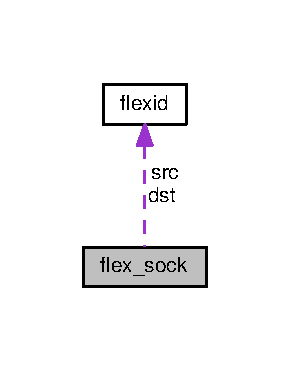
\includegraphics[width=139pt]{structflex__sock__coll__graph}
\end{center}
\end{figure}
\subsection*{Public Attributes}
\begin{DoxyCompactItemize}
\item 
struct sock \hyperlink{structflex__sock_a1ffc5042c0d6dd6b651ecb6a8e9b1096}{sk}
\item 
unsigned char \hyperlink{structflex__sock_acea083a0cc7f13d3491228dd261bfc70}{protocol}
\item 
short \hyperlink{structflex__sock_af4d0be6245faa22590e3d672d095a2a7}{message}
\item 
struct \hyperlink{structflexid}{flexid} \hyperlink{structflex__sock_a132b613c5f785e07196306bff98ef85d}{src}
\item 
struct \hyperlink{structflexid}{flexid} \hyperlink{structflex__sock_a1704e9612c290ef88bf674ea245b1835}{dst}
\item 
short \hyperlink{structflex__sock_afb460ef1d9e2fc1cc389ca5922f967d8}{addr\+\_\+type}
\item 
unsigned char \hyperlink{structflex__sock_a1c183d812ac68e320df127d58d303677}{addr\+\_\+len}
\item 
unsigned char \hyperlink{structflex__sock_a7c9d43f00ac325627f1396ffc10fe74a}{next\+\_\+hop} \mbox{[}M\+A\+X\+\_\+\+A\+D\+D\+R\+\_\+\+L\+EN\mbox{]}
\end{DoxyCompactItemize}


\subsection{Detailed Description}
The data structure for the Flex specified socket. 

\subsection{Member Data Documentation}
\index{flex\+\_\+sock@{flex\+\_\+sock}!addr\+\_\+len@{addr\+\_\+len}}
\index{addr\+\_\+len@{addr\+\_\+len}!flex\+\_\+sock@{flex\+\_\+sock}}
\subsubsection[{\texorpdfstring{addr\+\_\+len}{addr_len}}]{\setlength{\rightskip}{0pt plus 5cm}unsigned char flex\+\_\+sock\+::addr\+\_\+len}\hypertarget{structflex__sock_a1c183d812ac68e320df127d58d303677}{}\label{structflex__sock_a1c183d812ac68e320df127d58d303677}
The length of the address in the next hop \index{flex\+\_\+sock@{flex\+\_\+sock}!addr\+\_\+type@{addr\+\_\+type}}
\index{addr\+\_\+type@{addr\+\_\+type}!flex\+\_\+sock@{flex\+\_\+sock}}
\subsubsection[{\texorpdfstring{addr\+\_\+type}{addr_type}}]{\setlength{\rightskip}{0pt plus 5cm}short flex\+\_\+sock\+::addr\+\_\+type}\hypertarget{structflex__sock_afb460ef1d9e2fc1cc389ca5922f967d8}{}\label{structflex__sock_afb460ef1d9e2fc1cc389ca5922f967d8}
The address type of the next hop \index{flex\+\_\+sock@{flex\+\_\+sock}!dst@{dst}}
\index{dst@{dst}!flex\+\_\+sock@{flex\+\_\+sock}}
\subsubsection[{\texorpdfstring{dst}{dst}}]{\setlength{\rightskip}{0pt plus 5cm}struct {\bf flexid} flex\+\_\+sock\+::dst}\hypertarget{structflex__sock_a1704e9612c290ef88bf674ea245b1835}{}\label{structflex__sock_a1704e9612c290ef88bf674ea245b1835}
Flex ID of the destination \index{flex\+\_\+sock@{flex\+\_\+sock}!message@{message}}
\index{message@{message}!flex\+\_\+sock@{flex\+\_\+sock}}
\subsubsection[{\texorpdfstring{message}{message}}]{\setlength{\rightskip}{0pt plus 5cm}short flex\+\_\+sock\+::message}\hypertarget{structflex__sock_af4d0be6245faa22590e3d672d095a2a7}{}\label{structflex__sock_af4d0be6245faa22590e3d672d095a2a7}
The message type \index{flex\+\_\+sock@{flex\+\_\+sock}!next\+\_\+hop@{next\+\_\+hop}}
\index{next\+\_\+hop@{next\+\_\+hop}!flex\+\_\+sock@{flex\+\_\+sock}}
\subsubsection[{\texorpdfstring{next\+\_\+hop}{next_hop}}]{\setlength{\rightskip}{0pt plus 5cm}unsigned char flex\+\_\+sock\+::next\+\_\+hop\mbox{[}M\+A\+X\+\_\+\+A\+D\+D\+R\+\_\+\+L\+EN\mbox{]}}\hypertarget{structflex__sock_a7c9d43f00ac325627f1396ffc10fe74a}{}\label{structflex__sock_a7c9d43f00ac325627f1396ffc10fe74a}
The address of the next hop \index{flex\+\_\+sock@{flex\+\_\+sock}!protocol@{protocol}}
\index{protocol@{protocol}!flex\+\_\+sock@{flex\+\_\+sock}}
\subsubsection[{\texorpdfstring{protocol}{protocol}}]{\setlength{\rightskip}{0pt plus 5cm}unsigned char flex\+\_\+sock\+::protocol}\hypertarget{structflex__sock_acea083a0cc7f13d3491228dd261bfc70}{}\label{structflex__sock_acea083a0cc7f13d3491228dd261bfc70}
This member shows the reliable/unreliable communication is used \index{flex\+\_\+sock@{flex\+\_\+sock}!sk@{sk}}
\index{sk@{sk}!flex\+\_\+sock@{flex\+\_\+sock}}
\subsubsection[{\texorpdfstring{sk}{sk}}]{\setlength{\rightskip}{0pt plus 5cm}struct sock flex\+\_\+sock\+::sk}\hypertarget{structflex__sock_a1ffc5042c0d6dd6b651ecb6a8e9b1096}{}\label{structflex__sock_a1ffc5042c0d6dd6b651ecb6a8e9b1096}
This member contains the sock structure \index{flex\+\_\+sock@{flex\+\_\+sock}!src@{src}}
\index{src@{src}!flex\+\_\+sock@{flex\+\_\+sock}}
\subsubsection[{\texorpdfstring{src}{src}}]{\setlength{\rightskip}{0pt plus 5cm}struct {\bf flexid} flex\+\_\+sock\+::src}\hypertarget{structflex__sock_a132b613c5f785e07196306bff98ef85d}{}\label{structflex__sock_a132b613c5f785e07196306bff98ef85d}
Flex ID of the source 

The documentation for this struct was generated from the following file\+:\begin{DoxyCompactItemize}
\item 
socket/\hyperlink{flex__sock_8h}{flex\+\_\+sock.\+h}\end{DoxyCompactItemize}

\hypertarget{structflexhdr}{}\section{flexhdr Struct Reference}
\label{structflexhdr}\index{flexhdr@{flexhdr}}
\subsection*{Public Attributes}
\begin{DoxyCompactItemize}
\item 
\+\_\+\+\_\+u8 {\bfseries version}\hypertarget{structflexhdr_a58658c0c3ac88c2ae21cf52cdbeaefd0}{}\label{structflexhdr_a58658c0c3ac88c2ae21cf52cdbeaefd0}

\item 
\+\_\+\+\_\+u8 {\bfseries packet\+\_\+type}\hypertarget{structflexhdr_a3e17e4077f496e9eed85b5705a40b06f}{}\label{structflexhdr_a3e17e4077f496e9eed85b5705a40b06f}

\item 
\+\_\+\+\_\+u8 {\bfseries hash\+\_\+type}\hypertarget{structflexhdr_aa2a7292e9ff348680f83067955b58d0f}{}\label{structflexhdr_aa2a7292e9ff348680f83067955b58d0f}

\item 
\+\_\+\+\_\+u8 {\bfseries hop\+\_\+limit}\hypertarget{structflexhdr_a550e9254701dcd7665cdc1d52f9599fa}{}\label{structflexhdr_a550e9254701dcd7665cdc1d52f9599fa}

\item 
\+\_\+\+\_\+be16 {\bfseries header\+\_\+len}\hypertarget{structflexhdr_a7a2903458e61241565c61177a87c6dbb}{}\label{structflexhdr_a7a2903458e61241565c61177a87c6dbb}

\item 
\+\_\+\+\_\+sum16 {\bfseries check}\hypertarget{structflexhdr_a7e2d0c232c92ea39204ec52563cbd33e}{}\label{structflexhdr_a7e2d0c232c92ea39204ec52563cbd33e}

\item 
\+\_\+\+\_\+be16 {\bfseries packet\+\_\+id}\hypertarget{structflexhdr_a15281b3aa64868e176dffbb7ee5f2acc}{}\label{structflexhdr_a15281b3aa64868e176dffbb7ee5f2acc}

\item 
\+\_\+\+\_\+be16 {\bfseries frag\+\_\+off}\hypertarget{structflexhdr_a85f045e7acaf63edb2cd192266ef49bf}{}\label{structflexhdr_a85f045e7acaf63edb2cd192266ef49bf}

\item 
char {\bfseries sflex\+\_\+id} \mbox{[}F\+L\+E\+X\+\_\+\+I\+D\+\_\+\+L\+E\+N\+G\+TH\mbox{]}\hypertarget{structflexhdr_a3d0b687dac926a77cde8a5cc01f05533}{}\label{structflexhdr_a3d0b687dac926a77cde8a5cc01f05533}

\item 
char {\bfseries dflex\+\_\+id} \mbox{[}F\+L\+E\+X\+\_\+\+I\+D\+\_\+\+L\+E\+N\+G\+TH\mbox{]}\hypertarget{structflexhdr_aab2628ec55f6dedda9cd48de1677d49c}{}\label{structflexhdr_aab2628ec55f6dedda9cd48de1677d49c}

\item 
\+\_\+\+\_\+be16 {\bfseries packet\+\_\+len}\hypertarget{structflexhdr_a8e177eb08fa03f382eb67f75d9bf16b9}{}\label{structflexhdr_a8e177eb08fa03f382eb67f75d9bf16b9}

\item 
\+\_\+\+\_\+be32 {\bfseries seq}\hypertarget{structflexhdr_a1f437e344ae8752c7ea0586104bf67b4}{}\label{structflexhdr_a1f437e344ae8752c7ea0586104bf67b4}

\item 
\+\_\+\+\_\+be32 {\bfseries ack}\hypertarget{structflexhdr_a9504db4a12b79baa7937e1d11f521e57}{}\label{structflexhdr_a9504db4a12b79baa7937e1d11f521e57}

\end{DoxyCompactItemize}


The documentation for this struct was generated from the following files\+:\begin{DoxyCompactItemize}
\item 
apps/ipv4/proto\+\_\+flex.\+h\item 
include/flex/flex\+\_\+hdr.\+h\end{DoxyCompactItemize}

\hypertarget{structflexid}{}\section{flexid Struct Reference}
\label{structflexid}\index{flexid@{flexid}}


{\ttfamily \#include $<$flex\+\_\+id.\+h$>$}

\subsection*{Public Attributes}
\begin{DoxyCompactItemize}
\item 
\+\_\+\+\_\+u8 \hyperlink{structflexid_ab9e1df37109f8620f2be93955de9cb97}{identity} \mbox{[}20\mbox{]}
\item 
\+\_\+\+\_\+be32 \hyperlink{structflexid_a06122ad6fde6feb1e4edba60f476640e}{total\+\_\+segments}
\item 
\+\_\+\+\_\+be32 \hyperlink{structflexid_ae502fa12b4cd189628452ca8c6fd0dc0}{segment\+\_\+num}
\item 
\+\_\+\+\_\+be16 \hyperlink{structflexid_a652f4ff1a68f65a499f877337d4d7460}{length}
\end{DoxyCompactItemize}


\subsection{Member Data Documentation}
\index{flexid@{flexid}!identity@{identity}}
\index{identity@{identity}!flexid@{flexid}}
\subsubsection[{\texorpdfstring{identity}{identity}}]{\setlength{\rightskip}{0pt plus 5cm}\+\_\+\+\_\+u8 flexid\+::identity\mbox{[}20\mbox{]}}\hypertarget{structflexid_ab9e1df37109f8620f2be93955de9cb97}{}\label{structflexid_ab9e1df37109f8620f2be93955de9cb97}
\index{flexid@{flexid}!length@{length}}
\index{length@{length}!flexid@{flexid}}
\subsubsection[{\texorpdfstring{length}{length}}]{\setlength{\rightskip}{0pt plus 5cm}\+\_\+\+\_\+be16 flexid\+::length}\hypertarget{structflexid_a652f4ff1a68f65a499f877337d4d7460}{}\label{structflexid_a652f4ff1a68f65a499f877337d4d7460}
\index{flexid@{flexid}!segment\+\_\+num@{segment\+\_\+num}}
\index{segment\+\_\+num@{segment\+\_\+num}!flexid@{flexid}}
\subsubsection[{\texorpdfstring{segment\+\_\+num}{segment_num}}]{\setlength{\rightskip}{0pt plus 5cm}\+\_\+\+\_\+be32 flexid\+::segment\+\_\+num}\hypertarget{structflexid_ae502fa12b4cd189628452ca8c6fd0dc0}{}\label{structflexid_ae502fa12b4cd189628452ca8c6fd0dc0}
\index{flexid@{flexid}!total\+\_\+segments@{total\+\_\+segments}}
\index{total\+\_\+segments@{total\+\_\+segments}!flexid@{flexid}}
\subsubsection[{\texorpdfstring{total\+\_\+segments}{total_segments}}]{\setlength{\rightskip}{0pt plus 5cm}\+\_\+\+\_\+be32 flexid\+::total\+\_\+segments}\hypertarget{structflexid_a06122ad6fde6feb1e4edba60f476640e}{}\label{structflexid_a06122ad6fde6feb1e4edba60f476640e}


The documentation for this struct was generated from the following file\+:\begin{DoxyCompactItemize}
\item 
include/flex/\hyperlink{include_2flex_2flex__id_8h}{flex\+\_\+id.\+h}\end{DoxyCompactItemize}

\hypertarget{structflexidhdr}{}\section{flexidhdr Struct Reference}
\label{structflexidhdr}\index{flexidhdr@{flexidhdr}}


{\ttfamily \#include $<$flex\+\_\+id.\+h$>$}

\subsection*{Public Attributes}
\begin{DoxyCompactItemize}
\item 
uint8\+\_\+t \hyperlink{structflexidhdr_a040648453cb452e600995d86a1432264}{version}
\item 
uint8\+\_\+t \hyperlink{structflexidhdr_a0d1be6716bc037d0742bb7905c554b7d}{packet\+\_\+type}
\item 
uint8\+\_\+t \hyperlink{structflexidhdr_a4664d30de167966734c63a9602aa67d8}{hash\+\_\+type}
\item 
uint8\+\_\+t \hyperlink{structflexidhdr_ac0e058519cc822eb3cb525217bda557f}{hash\+\_\+len}
\item 
uint16\+\_\+t \hyperlink{structflexidhdr_a25cbbee361b8bff5511611a5f72cff57}{packet\+\_\+len}
\item 
uint16\+\_\+t \hyperlink{structflexidhdr_ae1825703c47432515e7eddb823e3489f}{checksum}
\item 
uint16\+\_\+t \hyperlink{structflexidhdr_a1fc7a84deb9e0042941f7c983f240691}{packet\+\_\+id}
\item 
uint16\+\_\+t \hyperlink{structflexidhdr_a7aa77d8aec125c11801198ca617e5ebe}{frag\+\_\+off}
\item 
uint16\+\_\+t \hyperlink{structflexidhdr_a1e5f6919e501e8aef925b4d78095ea06}{header\+\_\+len}
\item 
uint8\+\_\+t \hyperlink{structflexidhdr_a507914601558d094837046884f9b4d79}{hop\+\_\+limit}
\item 
uint8\+\_\+t \hyperlink{structflexidhdr_a79659668b865b2f14a1e5ac5e6ee63d5}{reserved}
\item 
uint8\+\_\+t $\ast$ \hyperlink{structflexidhdr_ae5f70fa4b298c9ff8fd8ac56d94f52ab}{saddr}
\item 
uint8\+\_\+t $\ast$ \hyperlink{structflexidhdr_a9eb9cfa99f8f77520244cd96d55145f5}{daddr}
\end{DoxyCompactItemize}


\subsection{Member Data Documentation}
\index{flexidhdr@{flexidhdr}!checksum@{checksum}}
\index{checksum@{checksum}!flexidhdr@{flexidhdr}}
\subsubsection[{\texorpdfstring{checksum}{checksum}}]{\setlength{\rightskip}{0pt plus 5cm}uint16\+\_\+t flexidhdr\+::checksum}\hypertarget{structflexidhdr_ae1825703c47432515e7eddb823e3489f}{}\label{structflexidhdr_ae1825703c47432515e7eddb823e3489f}
\index{flexidhdr@{flexidhdr}!daddr@{daddr}}
\index{daddr@{daddr}!flexidhdr@{flexidhdr}}
\subsubsection[{\texorpdfstring{daddr}{daddr}}]{\setlength{\rightskip}{0pt plus 5cm}uint8\+\_\+t$\ast$ flexidhdr\+::daddr}\hypertarget{structflexidhdr_a9eb9cfa99f8f77520244cd96d55145f5}{}\label{structflexidhdr_a9eb9cfa99f8f77520244cd96d55145f5}
\index{flexidhdr@{flexidhdr}!frag\+\_\+off@{frag\+\_\+off}}
\index{frag\+\_\+off@{frag\+\_\+off}!flexidhdr@{flexidhdr}}
\subsubsection[{\texorpdfstring{frag\+\_\+off}{frag_off}}]{\setlength{\rightskip}{0pt plus 5cm}uint16\+\_\+t flexidhdr\+::frag\+\_\+off}\hypertarget{structflexidhdr_a7aa77d8aec125c11801198ca617e5ebe}{}\label{structflexidhdr_a7aa77d8aec125c11801198ca617e5ebe}
\index{flexidhdr@{flexidhdr}!hash\+\_\+len@{hash\+\_\+len}}
\index{hash\+\_\+len@{hash\+\_\+len}!flexidhdr@{flexidhdr}}
\subsubsection[{\texorpdfstring{hash\+\_\+len}{hash_len}}]{\setlength{\rightskip}{0pt plus 5cm}uint8\+\_\+t flexidhdr\+::hash\+\_\+len}\hypertarget{structflexidhdr_ac0e058519cc822eb3cb525217bda557f}{}\label{structflexidhdr_ac0e058519cc822eb3cb525217bda557f}
\index{flexidhdr@{flexidhdr}!hash\+\_\+type@{hash\+\_\+type}}
\index{hash\+\_\+type@{hash\+\_\+type}!flexidhdr@{flexidhdr}}
\subsubsection[{\texorpdfstring{hash\+\_\+type}{hash_type}}]{\setlength{\rightskip}{0pt plus 5cm}uint8\+\_\+t flexidhdr\+::hash\+\_\+type}\hypertarget{structflexidhdr_a4664d30de167966734c63a9602aa67d8}{}\label{structflexidhdr_a4664d30de167966734c63a9602aa67d8}
\index{flexidhdr@{flexidhdr}!header\+\_\+len@{header\+\_\+len}}
\index{header\+\_\+len@{header\+\_\+len}!flexidhdr@{flexidhdr}}
\subsubsection[{\texorpdfstring{header\+\_\+len}{header_len}}]{\setlength{\rightskip}{0pt plus 5cm}uint16\+\_\+t flexidhdr\+::header\+\_\+len}\hypertarget{structflexidhdr_a1e5f6919e501e8aef925b4d78095ea06}{}\label{structflexidhdr_a1e5f6919e501e8aef925b4d78095ea06}
\index{flexidhdr@{flexidhdr}!hop\+\_\+limit@{hop\+\_\+limit}}
\index{hop\+\_\+limit@{hop\+\_\+limit}!flexidhdr@{flexidhdr}}
\subsubsection[{\texorpdfstring{hop\+\_\+limit}{hop_limit}}]{\setlength{\rightskip}{0pt plus 5cm}uint8\+\_\+t flexidhdr\+::hop\+\_\+limit}\hypertarget{structflexidhdr_a507914601558d094837046884f9b4d79}{}\label{structflexidhdr_a507914601558d094837046884f9b4d79}
\index{flexidhdr@{flexidhdr}!packet\+\_\+id@{packet\+\_\+id}}
\index{packet\+\_\+id@{packet\+\_\+id}!flexidhdr@{flexidhdr}}
\subsubsection[{\texorpdfstring{packet\+\_\+id}{packet_id}}]{\setlength{\rightskip}{0pt plus 5cm}uint16\+\_\+t flexidhdr\+::packet\+\_\+id}\hypertarget{structflexidhdr_a1fc7a84deb9e0042941f7c983f240691}{}\label{structflexidhdr_a1fc7a84deb9e0042941f7c983f240691}
\index{flexidhdr@{flexidhdr}!packet\+\_\+len@{packet\+\_\+len}}
\index{packet\+\_\+len@{packet\+\_\+len}!flexidhdr@{flexidhdr}}
\subsubsection[{\texorpdfstring{packet\+\_\+len}{packet_len}}]{\setlength{\rightskip}{0pt plus 5cm}uint16\+\_\+t flexidhdr\+::packet\+\_\+len}\hypertarget{structflexidhdr_a25cbbee361b8bff5511611a5f72cff57}{}\label{structflexidhdr_a25cbbee361b8bff5511611a5f72cff57}
\index{flexidhdr@{flexidhdr}!packet\+\_\+type@{packet\+\_\+type}}
\index{packet\+\_\+type@{packet\+\_\+type}!flexidhdr@{flexidhdr}}
\subsubsection[{\texorpdfstring{packet\+\_\+type}{packet_type}}]{\setlength{\rightskip}{0pt plus 5cm}uint8\+\_\+t flexidhdr\+::packet\+\_\+type}\hypertarget{structflexidhdr_a0d1be6716bc037d0742bb7905c554b7d}{}\label{structflexidhdr_a0d1be6716bc037d0742bb7905c554b7d}
\index{flexidhdr@{flexidhdr}!reserved@{reserved}}
\index{reserved@{reserved}!flexidhdr@{flexidhdr}}
\subsubsection[{\texorpdfstring{reserved}{reserved}}]{\setlength{\rightskip}{0pt plus 5cm}uint8\+\_\+t flexidhdr\+::reserved}\hypertarget{structflexidhdr_a79659668b865b2f14a1e5ac5e6ee63d5}{}\label{structflexidhdr_a79659668b865b2f14a1e5ac5e6ee63d5}
\index{flexidhdr@{flexidhdr}!saddr@{saddr}}
\index{saddr@{saddr}!flexidhdr@{flexidhdr}}
\subsubsection[{\texorpdfstring{saddr}{saddr}}]{\setlength{\rightskip}{0pt plus 5cm}uint8\+\_\+t$\ast$ flexidhdr\+::saddr}\hypertarget{structflexidhdr_ae5f70fa4b298c9ff8fd8ac56d94f52ab}{}\label{structflexidhdr_ae5f70fa4b298c9ff8fd8ac56d94f52ab}
\index{flexidhdr@{flexidhdr}!version@{version}}
\index{version@{version}!flexidhdr@{flexidhdr}}
\subsubsection[{\texorpdfstring{version}{version}}]{\setlength{\rightskip}{0pt plus 5cm}uint8\+\_\+t flexidhdr\+::version}\hypertarget{structflexidhdr_a040648453cb452e600995d86a1432264}{}\label{structflexidhdr_a040648453cb452e600995d86a1432264}


The documentation for this struct was generated from the following file\+:\begin{DoxyCompactItemize}
\item 
flexid/\hyperlink{flexid_2flex__id_8h}{flex\+\_\+id.\+h}\end{DoxyCompactItemize}

\hypertarget{structhash__entry}{}\section{hash\+\_\+entry Struct Reference}
\label{structhash__entry}\index{hash\+\_\+entry@{hash\+\_\+entry}}


{\ttfamily \#include $<$hash\+\_\+table.\+h$>$}



Collaboration diagram for hash\+\_\+entry\+:\nopagebreak
\begin{figure}[H]
\begin{center}
\leavevmode
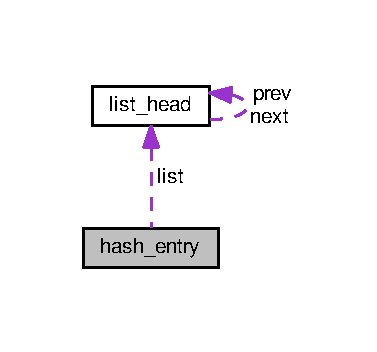
\includegraphics[width=181pt]{structhash__entry__coll__graph}
\end{center}
\end{figure}
\subsection*{Public Attributes}
\begin{DoxyCompactItemize}
\item 
struct \hyperlink{structlist__head}{list\+\_\+head} \hyperlink{structhash__entry_ada52d1b11e544cd19b58007cc3713069}{list}
\item 
unsigned char $\ast$ \hyperlink{structhash__entry_a0c23748b9dddd5f11b1ff9dbcbd47e9c}{key}
\item 
unsigned int \hyperlink{structhash__entry_a6f87c5657a590b7a848cc3f9a1d30d13}{keylen}
\end{DoxyCompactItemize}


\subsection{Member Data Documentation}
\index{hash\+\_\+entry@{hash\+\_\+entry}!key@{key}}
\index{key@{key}!hash\+\_\+entry@{hash\+\_\+entry}}
\subsubsection[{\texorpdfstring{key}{key}}]{\setlength{\rightskip}{0pt plus 5cm}unsigned char $\ast$ hash\+\_\+entry\+::key}\hypertarget{structhash__entry_a0c23748b9dddd5f11b1ff9dbcbd47e9c}{}\label{structhash__entry_a0c23748b9dddd5f11b1ff9dbcbd47e9c}
\index{hash\+\_\+entry@{hash\+\_\+entry}!keylen@{keylen}}
\index{keylen@{keylen}!hash\+\_\+entry@{hash\+\_\+entry}}
\subsubsection[{\texorpdfstring{keylen}{keylen}}]{\setlength{\rightskip}{0pt plus 5cm}unsigned int hash\+\_\+entry\+::keylen}\hypertarget{structhash__entry_a6f87c5657a590b7a848cc3f9a1d30d13}{}\label{structhash__entry_a6f87c5657a590b7a848cc3f9a1d30d13}
\index{hash\+\_\+entry@{hash\+\_\+entry}!list@{list}}
\index{list@{list}!hash\+\_\+entry@{hash\+\_\+entry}}
\subsubsection[{\texorpdfstring{list}{list}}]{\setlength{\rightskip}{0pt plus 5cm}struct {\bf list\+\_\+head} hash\+\_\+entry\+::list}\hypertarget{structhash__entry_ada52d1b11e544cd19b58007cc3713069}{}\label{structhash__entry_ada52d1b11e544cd19b58007cc3713069}


The documentation for this struct was generated from the following file\+:\begin{DoxyCompactItemize}
\item 
include/flex/\hyperlink{include_2flex_2hash__table_8h}{hash\+\_\+table.\+h}\end{DoxyCompactItemize}

\hypertarget{structhash__table}{}\section{hash\+\_\+table Struct Reference}
\label{structhash__table}\index{hash\+\_\+table@{hash\+\_\+table}}


{\ttfamily \#include $<$hash\+\_\+table.\+h$>$}



Collaboration diagram for hash\+\_\+table\+:\nopagebreak
\begin{figure}[H]
\begin{center}
\leavevmode
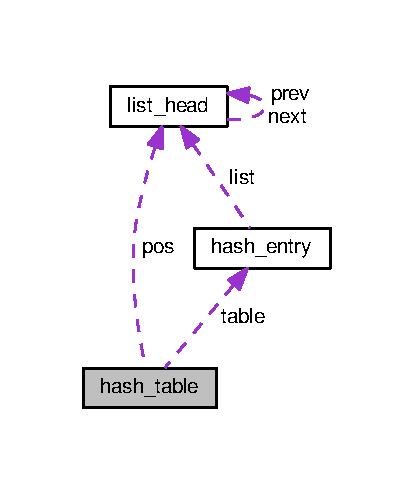
\includegraphics[width=199pt]{structhash__table__coll__graph}
\end{center}
\end{figure}
\subsection*{Public Attributes}
\begin{DoxyCompactItemize}
\item 
struct \hyperlink{structhash__entry}{hash\+\_\+entry} $\ast$ \hyperlink{structhash__table_a04cd18d2fc0ace3527670ceca050492b}{table}
\item 
unsigned int \hyperlink{structhash__table_a4678419b52c36e8b949b17eb4843a420}{buckets}
\item 
pthread\+\_\+mutex\+\_\+t $\ast$ \hyperlink{structhash__table_a4148c7a0d18b24d1c2961564dc0e7e7a}{bucket\+\_\+locks}
\item 
pthread\+\_\+mutex\+\_\+t \hyperlink{structhash__table_af4cefababf047c699eca5f45f8d4284e}{lock}
\item 
\hyperlink{util_2hash__table_8h_a9b0a83bb52986ea61f0e4351b66d41ef}{keycmp\+\_\+ptr} \hyperlink{structhash__table_a9465a319f391f0a50a4a84362c40fe48}{keycmp}
\item 
unsigned int \hyperlink{structhash__table_a77da69e21124ac1097627ae23ae72ef5}{\+\_\+\+\_\+ht\+\_\+i}
\item 
struct \hyperlink{structlist__head}{list\+\_\+head} $\ast$ \hyperlink{structhash__table_af9bcc20e562a8a4f6dd37aaa543a3883}{pos}
\end{DoxyCompactItemize}


\subsection{Member Data Documentation}
\index{hash\+\_\+table@{hash\+\_\+table}!\+\_\+\+\_\+ht\+\_\+i@{\+\_\+\+\_\+ht\+\_\+i}}
\index{\+\_\+\+\_\+ht\+\_\+i@{\+\_\+\+\_\+ht\+\_\+i}!hash\+\_\+table@{hash\+\_\+table}}
\subsubsection[{\texorpdfstring{\+\_\+\+\_\+ht\+\_\+i}{__ht_i}}]{\setlength{\rightskip}{0pt plus 5cm}unsigned int hash\+\_\+table\+::\+\_\+\+\_\+ht\+\_\+i}\hypertarget{structhash__table_a77da69e21124ac1097627ae23ae72ef5}{}\label{structhash__table_a77da69e21124ac1097627ae23ae72ef5}
\index{hash\+\_\+table@{hash\+\_\+table}!bucket\+\_\+locks@{bucket\+\_\+locks}}
\index{bucket\+\_\+locks@{bucket\+\_\+locks}!hash\+\_\+table@{hash\+\_\+table}}
\subsubsection[{\texorpdfstring{bucket\+\_\+locks}{bucket_locks}}]{\setlength{\rightskip}{0pt plus 5cm}pthread\+\_\+mutex\+\_\+t $\ast$ hash\+\_\+table\+::bucket\+\_\+locks}\hypertarget{structhash__table_a4148c7a0d18b24d1c2961564dc0e7e7a}{}\label{structhash__table_a4148c7a0d18b24d1c2961564dc0e7e7a}
\index{hash\+\_\+table@{hash\+\_\+table}!buckets@{buckets}}
\index{buckets@{buckets}!hash\+\_\+table@{hash\+\_\+table}}
\subsubsection[{\texorpdfstring{buckets}{buckets}}]{\setlength{\rightskip}{0pt plus 5cm}unsigned int hash\+\_\+table\+::buckets}\hypertarget{structhash__table_a4678419b52c36e8b949b17eb4843a420}{}\label{structhash__table_a4678419b52c36e8b949b17eb4843a420}
\index{hash\+\_\+table@{hash\+\_\+table}!keycmp@{keycmp}}
\index{keycmp@{keycmp}!hash\+\_\+table@{hash\+\_\+table}}
\subsubsection[{\texorpdfstring{keycmp}{keycmp}}]{\setlength{\rightskip}{0pt plus 5cm}{\bf keycmp\+\_\+ptr} hash\+\_\+table\+::keycmp}\hypertarget{structhash__table_a9465a319f391f0a50a4a84362c40fe48}{}\label{structhash__table_a9465a319f391f0a50a4a84362c40fe48}
\index{hash\+\_\+table@{hash\+\_\+table}!lock@{lock}}
\index{lock@{lock}!hash\+\_\+table@{hash\+\_\+table}}
\subsubsection[{\texorpdfstring{lock}{lock}}]{\setlength{\rightskip}{0pt plus 5cm}pthread\+\_\+mutex\+\_\+t hash\+\_\+table\+::lock}\hypertarget{structhash__table_af4cefababf047c699eca5f45f8d4284e}{}\label{structhash__table_af4cefababf047c699eca5f45f8d4284e}
\index{hash\+\_\+table@{hash\+\_\+table}!pos@{pos}}
\index{pos@{pos}!hash\+\_\+table@{hash\+\_\+table}}
\subsubsection[{\texorpdfstring{pos}{pos}}]{\setlength{\rightskip}{0pt plus 5cm}struct {\bf list\+\_\+head} $\ast$ hash\+\_\+table\+::pos}\hypertarget{structhash__table_af9bcc20e562a8a4f6dd37aaa543a3883}{}\label{structhash__table_af9bcc20e562a8a4f6dd37aaa543a3883}
\index{hash\+\_\+table@{hash\+\_\+table}!table@{table}}
\index{table@{table}!hash\+\_\+table@{hash\+\_\+table}}
\subsubsection[{\texorpdfstring{table}{table}}]{\setlength{\rightskip}{0pt plus 5cm}struct {\bf hash\+\_\+entry} $\ast$ hash\+\_\+table\+::table}\hypertarget{structhash__table_a04cd18d2fc0ace3527670ceca050492b}{}\label{structhash__table_a04cd18d2fc0ace3527670ceca050492b}


The documentation for this struct was generated from the following file\+:\begin{DoxyCompactItemize}
\item 
include/flex/\hyperlink{include_2flex_2hash__table_8h}{hash\+\_\+table.\+h}\end{DoxyCompactItemize}

\hypertarget{structid__manage__ops}{}\section{id\+\_\+manage\+\_\+ops Struct Reference}
\label{structid__manage__ops}\index{id\+\_\+manage\+\_\+ops@{id\+\_\+manage\+\_\+ops}}
\subsection*{Public Attributes}
\begin{DoxyCompactItemize}
\item 
int($\ast$ {\bfseries reg} )(\hyperlink{structflexid}{flexid\+\_\+t} $\ast$id)\hypertarget{structid__manage__ops_a1f5dd93a784407384a1cb31e34f212e2}{}\label{structid__manage__ops_a1f5dd93a784407384a1cb31e34f212e2}

\item 
int($\ast$ {\bfseries update} )(\hyperlink{structflexid}{flexid\+\_\+t} $\ast$id, unsigned char $\ast$key, unsigned char $\ast$value)\hypertarget{structid__manage__ops_a4a50cc4475967070b64333cfbc95b659}{}\label{structid__manage__ops_a4a50cc4475967070b64333cfbc95b659}

\item 
int($\ast$ {\bfseries request} )(\hyperlink{structflexid}{flexid\+\_\+t} $\ast$id)\hypertarget{structid__manage__ops_abd048ab844f857df4ffe671e6075770d}{}\label{structid__manage__ops_abd048ab844f857df4ffe671e6075770d}

\end{DoxyCompactItemize}


The documentation for this struct was generated from the following file\+:\begin{DoxyCompactItemize}
\item 
include/flex/id\+\_\+manage.\+h\end{DoxyCompactItemize}

\hypertarget{structlist__head}{}\section{list\+\_\+head Struct Reference}
\label{structlist__head}\index{list\+\_\+head@{list\+\_\+head}}


{\ttfamily \#include $<$list.\+h$>$}



Collaboration diagram for list\+\_\+head\+:\nopagebreak
\begin{figure}[H]
\begin{center}
\leavevmode
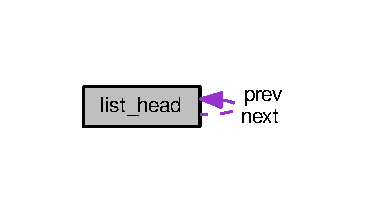
\includegraphics[width=176pt]{structlist__head__coll__graph}
\end{center}
\end{figure}
\subsection*{Public Attributes}
\begin{DoxyCompactItemize}
\item 
struct \hyperlink{structlist__head}{list\+\_\+head} $\ast$ \hyperlink{structlist__head_a44b2d28c78f7266869b3f00390bec772}{next}
\item 
struct \hyperlink{structlist__head}{list\+\_\+head} $\ast$ \hyperlink{structlist__head_aaa0eabda8877e1d6de73a33f223ad004}{prev}
\end{DoxyCompactItemize}


\subsection{Member Data Documentation}
\index{list\+\_\+head@{list\+\_\+head}!next@{next}}
\index{next@{next}!list\+\_\+head@{list\+\_\+head}}
\subsubsection[{\texorpdfstring{next}{next}}]{\setlength{\rightskip}{0pt plus 5cm}struct {\bf list\+\_\+head} $\ast$ list\+\_\+head\+::next}\hypertarget{structlist__head_a44b2d28c78f7266869b3f00390bec772}{}\label{structlist__head_a44b2d28c78f7266869b3f00390bec772}
\index{list\+\_\+head@{list\+\_\+head}!prev@{prev}}
\index{prev@{prev}!list\+\_\+head@{list\+\_\+head}}
\subsubsection[{\texorpdfstring{prev}{prev}}]{\setlength{\rightskip}{0pt plus 5cm}struct {\bf list\+\_\+head} $\ast$ list\+\_\+head\+::prev}\hypertarget{structlist__head_aaa0eabda8877e1d6de73a33f223ad004}{}\label{structlist__head_aaa0eabda8877e1d6de73a33f223ad004}


The documentation for this struct was generated from the following file\+:\begin{DoxyCompactItemize}
\item 
include/flex/\hyperlink{include_2flex_2list_8h}{list.\+h}\end{DoxyCompactItemize}

\hypertarget{structquery__list}{}\section{query\+\_\+list Struct Reference}
\label{structquery__list}\index{query\+\_\+list@{query\+\_\+list}}


The documentation for this struct was generated from the following file\+:\begin{DoxyCompactItemize}
\item 
include/flex/flex\+\_\+query.\+h\end{DoxyCompactItemize}

\hypertarget{structreply__list}{}\section{reply\+\_\+list Struct Reference}
\label{structreply__list}\index{reply\+\_\+list@{reply\+\_\+list}}


The documentation for this struct was generated from the following file\+:\begin{DoxyCompactItemize}
\item 
include/flex/flex\+\_\+query.\+h\end{DoxyCompactItemize}

\hypertarget{structrepo}{}\section{repo Struct Reference}
\label{structrepo}\index{repo@{repo}}


The documentation for this struct was generated from the following file\+:\begin{DoxyCompactItemize}
\item 
include/flex/flex\+\_\+repo.\+h\end{DoxyCompactItemize}

\hypertarget{structresponse}{}\section{response Struct Reference}
\label{structresponse}\index{response@{response}}


{\ttfamily \#include $<$flex\+\_\+request.\+h$>$}

\subsection*{Public Attributes}
\begin{DoxyCompactItemize}
\item 
short \hyperlink{structresponse_ae098504ec8fd2c1eafd3b8487a783575}{error}
\item 
short \hyperlink{structresponse_a2f45198ba85a80efc09cbde6098af0b8}{addr\+\_\+type}
\item 
unsigned char \hyperlink{structresponse_a835f830c6f09ed6b0e702b3021f66a57}{addr\+\_\+len}
\item 
unsigned char \hyperlink{structresponse_a6b7eac313932e975cd88a0d998867bb3}{next\+\_\+hop} \mbox{[}\hyperlink{flex__addr_8h_a13b71bf0266170fc990217b80b27f40d}{M\+A\+X\+\_\+\+A\+D\+D\+R\+E\+S\+S\+\_\+\+L\+E\+N\+G\+TH}\mbox{]}
\end{DoxyCompactItemize}


\subsection{Member Data Documentation}
\index{response@{response}!addr\+\_\+len@{addr\+\_\+len}}
\index{addr\+\_\+len@{addr\+\_\+len}!response@{response}}
\subsubsection[{\texorpdfstring{addr\+\_\+len}{addr_len}}]{\setlength{\rightskip}{0pt plus 5cm}unsigned char response\+::addr\+\_\+len}\hypertarget{structresponse_a835f830c6f09ed6b0e702b3021f66a57}{}\label{structresponse_a835f830c6f09ed6b0e702b3021f66a57}
\index{response@{response}!addr\+\_\+type@{addr\+\_\+type}}
\index{addr\+\_\+type@{addr\+\_\+type}!response@{response}}
\subsubsection[{\texorpdfstring{addr\+\_\+type}{addr_type}}]{\setlength{\rightskip}{0pt plus 5cm}short response\+::addr\+\_\+type}\hypertarget{structresponse_a2f45198ba85a80efc09cbde6098af0b8}{}\label{structresponse_a2f45198ba85a80efc09cbde6098af0b8}
\index{response@{response}!error@{error}}
\index{error@{error}!response@{response}}
\subsubsection[{\texorpdfstring{error}{error}}]{\setlength{\rightskip}{0pt plus 5cm}short response\+::error}\hypertarget{structresponse_ae098504ec8fd2c1eafd3b8487a783575}{}\label{structresponse_ae098504ec8fd2c1eafd3b8487a783575}
\index{response@{response}!next\+\_\+hop@{next\+\_\+hop}}
\index{next\+\_\+hop@{next\+\_\+hop}!response@{response}}
\subsubsection[{\texorpdfstring{next\+\_\+hop}{next_hop}}]{\setlength{\rightskip}{0pt plus 5cm}unsigned char response\+::next\+\_\+hop\mbox{[}{\bf M\+A\+X\+\_\+\+A\+D\+D\+R\+E\+S\+S\+\_\+\+L\+E\+N\+G\+TH}\mbox{]}}\hypertarget{structresponse_a6b7eac313932e975cd88a0d998867bb3}{}\label{structresponse_a6b7eac313932e975cd88a0d998867bb3}


The documentation for this struct was generated from the following file\+:\begin{DoxyCompactItemize}
\item 
include/flex/\hyperlink{flex__request_8h}{flex\+\_\+request.\+h}\end{DoxyCompactItemize}

\hypertarget{structrflexhdr}{}\section{rflexhdr Struct Reference}
\label{structrflexhdr}\index{rflexhdr@{rflexhdr}}


Collaboration diagram for rflexhdr\+:\nopagebreak
\begin{figure}[H]
\begin{center}
\leavevmode
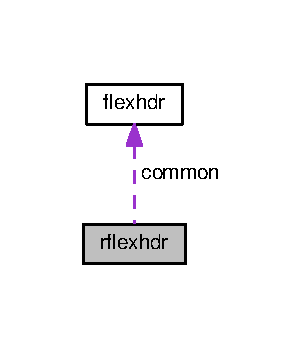
\includegraphics[width=146pt]{structrflexhdr__coll__graph}
\end{center}
\end{figure}
\subsection*{Public Attributes}
\begin{DoxyCompactItemize}
\item 
struct \hyperlink{structflexhdr}{flexhdr} {\bfseries common}\hypertarget{structrflexhdr_a0e80ead5eb57aba13d18f75f0906569c}{}\label{structrflexhdr_a0e80ead5eb57aba13d18f75f0906569c}

\item 
char {\bfseries sflex\+\_\+id} \mbox{[}F\+L\+E\+X\+\_\+\+I\+D\+\_\+\+L\+E\+N\+G\+TH\mbox{]}\hypertarget{structrflexhdr_aa79b53451e65228d567880e512cadc3e}{}\label{structrflexhdr_aa79b53451e65228d567880e512cadc3e}

\item 
char {\bfseries dflex\+\_\+id} \mbox{[}F\+L\+E\+X\+\_\+\+I\+D\+\_\+\+L\+E\+N\+G\+TH\mbox{]}\hypertarget{structrflexhdr_a091799a62ae442e024334d0eb4cb86b6}{}\label{structrflexhdr_a091799a62ae442e024334d0eb4cb86b6}

\item 
\+\_\+\+\_\+be16 {\bfseries packet\+\_\+len}\hypertarget{structrflexhdr_a2cc8c14fec43032de69ef360ffc4dfbe}{}\label{structrflexhdr_a2cc8c14fec43032de69ef360ffc4dfbe}

\item 
\+\_\+\+\_\+be32 {\bfseries seq}\hypertarget{structrflexhdr_a5ef194bf9db68ec8f6b050ca9608bd75}{}\label{structrflexhdr_a5ef194bf9db68ec8f6b050ca9608bd75}

\item 
\+\_\+\+\_\+be32 {\bfseries ack}\hypertarget{structrflexhdr_ae799b07034366e7e68c5b441f816e183}{}\label{structrflexhdr_ae799b07034366e7e68c5b441f816e183}

\end{DoxyCompactItemize}


The documentation for this struct was generated from the following file\+:\begin{DoxyCompactItemize}
\item 
include/flex/flex\+\_\+hdr.\+h\end{DoxyCompactItemize}

\hypertarget{structrflexhdr__ext}{}\section{rflexhdr\+\_\+ext Struct Reference}
\label{structrflexhdr__ext}\index{rflexhdr\+\_\+ext@{rflexhdr\+\_\+ext}}


Collaboration diagram for rflexhdr\+\_\+ext\+:\nopagebreak
\begin{figure}[H]
\begin{center}
\leavevmode
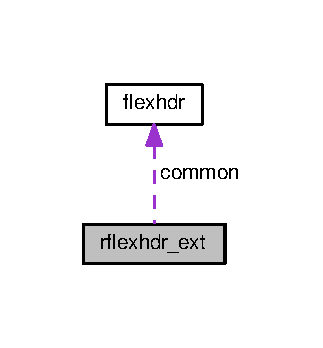
\includegraphics[width=155pt]{structrflexhdr__ext__coll__graph}
\end{center}
\end{figure}
\subsection*{Public Attributes}
\begin{DoxyCompactItemize}
\item 
struct \hyperlink{structflexhdr}{flexhdr} {\bfseries common}\hypertarget{structrflexhdr__ext_ac57a5553651d7cdde22b2d00c0a916ce}{}\label{structrflexhdr__ext_ac57a5553651d7cdde22b2d00c0a916ce}

\item 
char {\bfseries sflex\+\_\+id} \mbox{[}F\+L\+E\+X\+\_\+\+I\+D\+\_\+\+E\+X\+T\+\_\+\+L\+E\+N\+G\+TH\mbox{]}\hypertarget{structrflexhdr__ext_aba2b1333b35892ce3ae9c75dd8e2a521}{}\label{structrflexhdr__ext_aba2b1333b35892ce3ae9c75dd8e2a521}

\item 
char {\bfseries dflex\+\_\+id} \mbox{[}F\+L\+E\+X\+\_\+\+I\+D\+\_\+\+E\+X\+T\+\_\+\+L\+E\+N\+G\+TH\mbox{]}\hypertarget{structrflexhdr__ext_a3e35c1161803908776955800eb2ad3fe}{}\label{structrflexhdr__ext_a3e35c1161803908776955800eb2ad3fe}

\item 
\+\_\+\+\_\+be16 {\bfseries packet\+\_\+len}\hypertarget{structrflexhdr__ext_ac716297c579ced38da559cf53967f09b}{}\label{structrflexhdr__ext_ac716297c579ced38da559cf53967f09b}

\item 
\+\_\+\+\_\+be32 {\bfseries seq}\hypertarget{structrflexhdr__ext_a240fcbc0eff91a233304845f516d75d8}{}\label{structrflexhdr__ext_a240fcbc0eff91a233304845f516d75d8}

\item 
\+\_\+\+\_\+be32 {\bfseries ack}\hypertarget{structrflexhdr__ext_aee0018851d2f3381fd99c405606731b4}{}\label{structrflexhdr__ext_aee0018851d2f3381fd99c405606731b4}

\end{DoxyCompactItemize}


The documentation for this struct was generated from the following file\+:\begin{DoxyCompactItemize}
\item 
include/flex/flex\+\_\+hdr.\+h\end{DoxyCompactItemize}

\hypertarget{structsockaddr__flex}{}\section{sockaddr\+\_\+flex Struct Reference}
\label{structsockaddr__flex}\index{sockaddr\+\_\+flex@{sockaddr\+\_\+flex}}


{\ttfamily \#include $<$flex\+\_\+socket.\+h$>$}



Collaboration diagram for sockaddr\+\_\+flex\+:\nopagebreak
\begin{figure}[H]
\begin{center}
\leavevmode
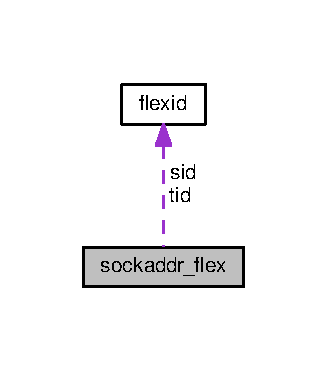
\includegraphics[width=157pt]{structsockaddr__flex__coll__graph}
\end{center}
\end{figure}
\subsection*{Public Attributes}
\begin{DoxyCompactItemize}
\item 
\+\_\+\+\_\+kernel\+\_\+sa\+\_\+family\+\_\+t \hyperlink{structsockaddr__flex_a0bebb0734429c3e6a548fc61de27c9c0}{sin\+\_\+family}
\item 
struct \hyperlink{structflexid}{flexid} \hyperlink{structsockaddr__flex_ae2d332f61042d379e3521f7e42603037}{sid}
\item 
struct \hyperlink{structflexid}{flexid} \hyperlink{structsockaddr__flex_a841742293b927751d2c0f8c48d7a5828}{tid}
\item 
short \hyperlink{structsockaddr__flex_ac1581ee2d027808218f3173c372924a1}{message}
\item 
short \hyperlink{structsockaddr__flex_a8945354761455603e8f09077e454defe}{addr\+\_\+type}
\item 
unsigned char \hyperlink{structsockaddr__flex_a44a4c4cabcecc77838283ed0a2fe22bb}{addr\+\_\+len}
\item 
unsigned char \hyperlink{structsockaddr__flex_a6869850bbb4ae164d955372332fffee3}{next\+\_\+hop} \mbox{[}\hyperlink{flex__addr_8h_a13b71bf0266170fc990217b80b27f40d}{M\+A\+X\+\_\+\+A\+D\+D\+R\+E\+S\+S\+\_\+\+L\+E\+N\+G\+TH}\mbox{]}
\end{DoxyCompactItemize}


\subsection{Member Data Documentation}
\index{sockaddr\+\_\+flex@{sockaddr\+\_\+flex}!addr\+\_\+len@{addr\+\_\+len}}
\index{addr\+\_\+len@{addr\+\_\+len}!sockaddr\+\_\+flex@{sockaddr\+\_\+flex}}
\subsubsection[{\texorpdfstring{addr\+\_\+len}{addr_len}}]{\setlength{\rightskip}{0pt plus 5cm}unsigned char sockaddr\+\_\+flex\+::addr\+\_\+len}\hypertarget{structsockaddr__flex_a44a4c4cabcecc77838283ed0a2fe22bb}{}\label{structsockaddr__flex_a44a4c4cabcecc77838283ed0a2fe22bb}
\index{sockaddr\+\_\+flex@{sockaddr\+\_\+flex}!addr\+\_\+type@{addr\+\_\+type}}
\index{addr\+\_\+type@{addr\+\_\+type}!sockaddr\+\_\+flex@{sockaddr\+\_\+flex}}
\subsubsection[{\texorpdfstring{addr\+\_\+type}{addr_type}}]{\setlength{\rightskip}{0pt plus 5cm}short sockaddr\+\_\+flex\+::addr\+\_\+type}\hypertarget{structsockaddr__flex_a8945354761455603e8f09077e454defe}{}\label{structsockaddr__flex_a8945354761455603e8f09077e454defe}
\index{sockaddr\+\_\+flex@{sockaddr\+\_\+flex}!message@{message}}
\index{message@{message}!sockaddr\+\_\+flex@{sockaddr\+\_\+flex}}
\subsubsection[{\texorpdfstring{message}{message}}]{\setlength{\rightskip}{0pt plus 5cm}short sockaddr\+\_\+flex\+::message}\hypertarget{structsockaddr__flex_ac1581ee2d027808218f3173c372924a1}{}\label{structsockaddr__flex_ac1581ee2d027808218f3173c372924a1}
\index{sockaddr\+\_\+flex@{sockaddr\+\_\+flex}!next\+\_\+hop@{next\+\_\+hop}}
\index{next\+\_\+hop@{next\+\_\+hop}!sockaddr\+\_\+flex@{sockaddr\+\_\+flex}}
\subsubsection[{\texorpdfstring{next\+\_\+hop}{next_hop}}]{\setlength{\rightskip}{0pt plus 5cm}unsigned char sockaddr\+\_\+flex\+::next\+\_\+hop\mbox{[}{\bf M\+A\+X\+\_\+\+A\+D\+D\+R\+E\+S\+S\+\_\+\+L\+E\+N\+G\+TH}\mbox{]}}\hypertarget{structsockaddr__flex_a6869850bbb4ae164d955372332fffee3}{}\label{structsockaddr__flex_a6869850bbb4ae164d955372332fffee3}
\index{sockaddr\+\_\+flex@{sockaddr\+\_\+flex}!sid@{sid}}
\index{sid@{sid}!sockaddr\+\_\+flex@{sockaddr\+\_\+flex}}
\subsubsection[{\texorpdfstring{sid}{sid}}]{\setlength{\rightskip}{0pt plus 5cm}struct {\bf flexid} sockaddr\+\_\+flex\+::sid}\hypertarget{structsockaddr__flex_ae2d332f61042d379e3521f7e42603037}{}\label{structsockaddr__flex_ae2d332f61042d379e3521f7e42603037}
\index{sockaddr\+\_\+flex@{sockaddr\+\_\+flex}!sin\+\_\+family@{sin\+\_\+family}}
\index{sin\+\_\+family@{sin\+\_\+family}!sockaddr\+\_\+flex@{sockaddr\+\_\+flex}}
\subsubsection[{\texorpdfstring{sin\+\_\+family}{sin_family}}]{\setlength{\rightskip}{0pt plus 5cm}\+\_\+\+\_\+kernel\+\_\+sa\+\_\+family\+\_\+t sockaddr\+\_\+flex\+::sin\+\_\+family}\hypertarget{structsockaddr__flex_a0bebb0734429c3e6a548fc61de27c9c0}{}\label{structsockaddr__flex_a0bebb0734429c3e6a548fc61de27c9c0}
\index{sockaddr\+\_\+flex@{sockaddr\+\_\+flex}!tid@{tid}}
\index{tid@{tid}!sockaddr\+\_\+flex@{sockaddr\+\_\+flex}}
\subsubsection[{\texorpdfstring{tid}{tid}}]{\setlength{\rightskip}{0pt plus 5cm}struct {\bf flexid} sockaddr\+\_\+flex\+::tid}\hypertarget{structsockaddr__flex_a841742293b927751d2c0f8c48d7a5828}{}\label{structsockaddr__flex_a841742293b927751d2c0f8c48d7a5828}


The documentation for this struct was generated from the following file\+:\begin{DoxyCompactItemize}
\item 
include/flex/\hyperlink{flex__socket_8h}{flex\+\_\+socket.\+h}\end{DoxyCompactItemize}

\hypertarget{structu__hslot}{}\section{u\+\_\+hslot Struct Reference}
\label{structu__hslot}\index{u\+\_\+hslot@{u\+\_\+hslot}}
\subsection*{Public Attributes}
\begin{DoxyCompactItemize}
\item 
struct hlist\+\_\+nulls\+\_\+head {\bfseries head}\hypertarget{structu__hslot_abe6060ce741ff9e94d6f4669ec7f4c9a}{}\label{structu__hslot_abe6060ce741ff9e94d6f4669ec7f4c9a}

\item 
int {\bfseries count}\hypertarget{structu__hslot_a2eee707762aa72c4d82f24d0422efa19}{}\label{structu__hslot_a2eee707762aa72c4d82f24d0422efa19}

\item 
spinlock\+\_\+t {\bfseries lock}\hypertarget{structu__hslot_a3a866b196889821639c6d1aa91af6154}{}\label{structu__hslot_a3a866b196889821639c6d1aa91af6154}

\end{DoxyCompactItemize}


The documentation for this struct was generated from the following file\+:\begin{DoxyCompactItemize}
\item 
socket/flex\+\_\+unreliable.\+h\end{DoxyCompactItemize}

\hypertarget{structu__table}{}\section{u\+\_\+table Struct Reference}
\label{structu__table}\index{u\+\_\+table@{u\+\_\+table}}


{\ttfamily \#include $<$flex\+\_\+unreliable.\+h$>$}



Collaboration diagram for u\+\_\+table\+:\nopagebreak
\begin{figure}[H]
\begin{center}
\leavevmode
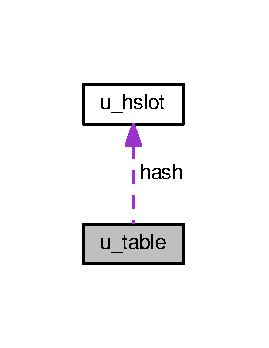
\includegraphics[width=129pt]{structu__table__coll__graph}
\end{center}
\end{figure}
\subsection*{Public Attributes}
\begin{DoxyCompactItemize}
\item 
struct \hyperlink{structu__hslot}{u\+\_\+hslot} $\ast$ \hyperlink{structu__table_a9d4512b1f9f38f0a6a24841ce2ca32a6}{hash}
\item 
unsigned int \hyperlink{structu__table_aeb1108e804777cac0e332f0310a78f09}{mask}
\item 
unsigned int \hyperlink{structu__table_ab9c33f2ba15bf3544b0176fbe59ccecd}{log}
\end{DoxyCompactItemize}


\subsection{Member Data Documentation}
\index{u\+\_\+table@{u\+\_\+table}!hash@{hash}}
\index{hash@{hash}!u\+\_\+table@{u\+\_\+table}}
\subsubsection[{\texorpdfstring{hash}{hash}}]{\setlength{\rightskip}{0pt plus 5cm}struct {\bf u\+\_\+hslot}$\ast$ u\+\_\+table\+::hash}\hypertarget{structu__table_a9d4512b1f9f38f0a6a24841ce2ca32a6}{}\label{structu__table_a9d4512b1f9f38f0a6a24841ce2ca32a6}
\index{u\+\_\+table@{u\+\_\+table}!log@{log}}
\index{log@{log}!u\+\_\+table@{u\+\_\+table}}
\subsubsection[{\texorpdfstring{log}{log}}]{\setlength{\rightskip}{0pt plus 5cm}unsigned int u\+\_\+table\+::log}\hypertarget{structu__table_ab9c33f2ba15bf3544b0176fbe59ccecd}{}\label{structu__table_ab9c33f2ba15bf3544b0176fbe59ccecd}
\index{u\+\_\+table@{u\+\_\+table}!mask@{mask}}
\index{mask@{mask}!u\+\_\+table@{u\+\_\+table}}
\subsubsection[{\texorpdfstring{mask}{mask}}]{\setlength{\rightskip}{0pt plus 5cm}unsigned int u\+\_\+table\+::mask}\hypertarget{structu__table_aeb1108e804777cac0e332f0310a78f09}{}\label{structu__table_aeb1108e804777cac0e332f0310a78f09}


The documentation for this struct was generated from the following file\+:\begin{DoxyCompactItemize}
\item 
socket/\hyperlink{flex__unreliable_8h}{flex\+\_\+unreliable.\+h}\end{DoxyCompactItemize}

\hypertarget{structuflexhdr}{}\section{uflexhdr Struct Reference}
\label{structuflexhdr}\index{uflexhdr@{uflexhdr}}


{\ttfamily \#include $<$flex\+\_\+hdr.\+h$>$}



Collaboration diagram for uflexhdr\+:\nopagebreak
\begin{figure}[H]
\begin{center}
\leavevmode
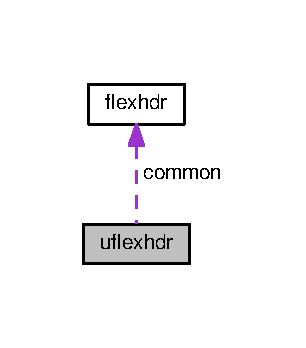
\includegraphics[width=147pt]{structuflexhdr__coll__graph}
\end{center}
\end{figure}
\subsection*{Public Attributes}
\begin{DoxyCompactItemize}
\item 
struct \hyperlink{structflexhdr}{flexhdr} \hyperlink{structuflexhdr_a298ecaecd1223467c1820a652458cff9}{common}
\item 
char \hyperlink{structuflexhdr_a359db5a95d160b5bacdde8883a9d1ee7}{sflex\+\_\+id} \mbox{[}\hyperlink{flex__const_8h_a342f27a8d723d83c803e6d934f999ada}{F\+L\+E\+X\+\_\+\+I\+D\+\_\+\+L\+E\+N\+G\+TH}\mbox{]}
\item 
char \hyperlink{structuflexhdr_a8733c5298ef2cdefd132ecec4878605f}{dflex\+\_\+id} \mbox{[}\hyperlink{flex__const_8h_a342f27a8d723d83c803e6d934f999ada}{F\+L\+E\+X\+\_\+\+I\+D\+\_\+\+L\+E\+N\+G\+TH}\mbox{]}
\item 
\+\_\+\+\_\+be16 \hyperlink{structuflexhdr_a633f53e21cbca9248040e940553af36e}{packet\+\_\+len}
\end{DoxyCompactItemize}


\subsection{Member Data Documentation}
\index{uflexhdr@{uflexhdr}!common@{common}}
\index{common@{common}!uflexhdr@{uflexhdr}}
\subsubsection[{\texorpdfstring{common}{common}}]{\setlength{\rightskip}{0pt plus 5cm}struct {\bf flexhdr} uflexhdr\+::common}\hypertarget{structuflexhdr_a298ecaecd1223467c1820a652458cff9}{}\label{structuflexhdr_a298ecaecd1223467c1820a652458cff9}
\index{uflexhdr@{uflexhdr}!dflex\+\_\+id@{dflex\+\_\+id}}
\index{dflex\+\_\+id@{dflex\+\_\+id}!uflexhdr@{uflexhdr}}
\subsubsection[{\texorpdfstring{dflex\+\_\+id}{dflex_id}}]{\setlength{\rightskip}{0pt plus 5cm}char uflexhdr\+::dflex\+\_\+id\mbox{[}{\bf F\+L\+E\+X\+\_\+\+I\+D\+\_\+\+L\+E\+N\+G\+TH}\mbox{]}}\hypertarget{structuflexhdr_a8733c5298ef2cdefd132ecec4878605f}{}\label{structuflexhdr_a8733c5298ef2cdefd132ecec4878605f}
\index{uflexhdr@{uflexhdr}!packet\+\_\+len@{packet\+\_\+len}}
\index{packet\+\_\+len@{packet\+\_\+len}!uflexhdr@{uflexhdr}}
\subsubsection[{\texorpdfstring{packet\+\_\+len}{packet_len}}]{\setlength{\rightskip}{0pt plus 5cm}\+\_\+\+\_\+be16 uflexhdr\+::packet\+\_\+len}\hypertarget{structuflexhdr_a633f53e21cbca9248040e940553af36e}{}\label{structuflexhdr_a633f53e21cbca9248040e940553af36e}
\index{uflexhdr@{uflexhdr}!sflex\+\_\+id@{sflex\+\_\+id}}
\index{sflex\+\_\+id@{sflex\+\_\+id}!uflexhdr@{uflexhdr}}
\subsubsection[{\texorpdfstring{sflex\+\_\+id}{sflex_id}}]{\setlength{\rightskip}{0pt plus 5cm}char uflexhdr\+::sflex\+\_\+id\mbox{[}{\bf F\+L\+E\+X\+\_\+\+I\+D\+\_\+\+L\+E\+N\+G\+TH}\mbox{]}}\hypertarget{structuflexhdr_a359db5a95d160b5bacdde8883a9d1ee7}{}\label{structuflexhdr_a359db5a95d160b5bacdde8883a9d1ee7}


The documentation for this struct was generated from the following file\+:\begin{DoxyCompactItemize}
\item 
include/flex/\hyperlink{flex__hdr_8h}{flex\+\_\+hdr.\+h}\end{DoxyCompactItemize}

\hypertarget{structuflexhdr__ext}{}\section{uflexhdr\+\_\+ext Struct Reference}
\label{structuflexhdr__ext}\index{uflexhdr\+\_\+ext@{uflexhdr\+\_\+ext}}


{\ttfamily \#include $<$flex\+\_\+hdr.\+h$>$}



Collaboration diagram for uflexhdr\+\_\+ext\+:\nopagebreak
\begin{figure}[H]
\begin{center}
\leavevmode
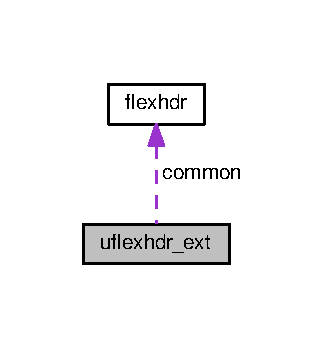
\includegraphics[width=156pt]{structuflexhdr__ext__coll__graph}
\end{center}
\end{figure}
\subsection*{Public Attributes}
\begin{DoxyCompactItemize}
\item 
struct \hyperlink{structflexhdr}{flexhdr} \hyperlink{structuflexhdr__ext_af481d03a7524a0f483e6fd8877c00563}{common}
\item 
char \hyperlink{structuflexhdr__ext_abf9a4c10efddc6b46acf9e25915cdcb3}{sflex\+\_\+id} \mbox{[}\hyperlink{flex__const_8h_a5bfdaffe9863d3fcfc3b90fa2a893bfd}{F\+L\+E\+X\+\_\+\+I\+D\+\_\+\+E\+X\+T\+\_\+\+L\+E\+N\+G\+TH}\mbox{]}
\item 
char \hyperlink{structuflexhdr__ext_a61d75d5fd362fb576a53fa8f973c2380}{dflex\+\_\+id} \mbox{[}\hyperlink{flex__const_8h_a5bfdaffe9863d3fcfc3b90fa2a893bfd}{F\+L\+E\+X\+\_\+\+I\+D\+\_\+\+E\+X\+T\+\_\+\+L\+E\+N\+G\+TH}\mbox{]}
\item 
\+\_\+\+\_\+be16 \hyperlink{structuflexhdr__ext_aa8dd1115a6af281d1a91102926d5cd4d}{packet\+\_\+len}
\end{DoxyCompactItemize}


\subsection{Member Data Documentation}
\index{uflexhdr\+\_\+ext@{uflexhdr\+\_\+ext}!common@{common}}
\index{common@{common}!uflexhdr\+\_\+ext@{uflexhdr\+\_\+ext}}
\subsubsection[{\texorpdfstring{common}{common}}]{\setlength{\rightskip}{0pt plus 5cm}struct {\bf flexhdr} uflexhdr\+\_\+ext\+::common}\hypertarget{structuflexhdr__ext_af481d03a7524a0f483e6fd8877c00563}{}\label{structuflexhdr__ext_af481d03a7524a0f483e6fd8877c00563}
\index{uflexhdr\+\_\+ext@{uflexhdr\+\_\+ext}!dflex\+\_\+id@{dflex\+\_\+id}}
\index{dflex\+\_\+id@{dflex\+\_\+id}!uflexhdr\+\_\+ext@{uflexhdr\+\_\+ext}}
\subsubsection[{\texorpdfstring{dflex\+\_\+id}{dflex_id}}]{\setlength{\rightskip}{0pt plus 5cm}char uflexhdr\+\_\+ext\+::dflex\+\_\+id\mbox{[}{\bf F\+L\+E\+X\+\_\+\+I\+D\+\_\+\+E\+X\+T\+\_\+\+L\+E\+N\+G\+TH}\mbox{]}}\hypertarget{structuflexhdr__ext_a61d75d5fd362fb576a53fa8f973c2380}{}\label{structuflexhdr__ext_a61d75d5fd362fb576a53fa8f973c2380}
\index{uflexhdr\+\_\+ext@{uflexhdr\+\_\+ext}!packet\+\_\+len@{packet\+\_\+len}}
\index{packet\+\_\+len@{packet\+\_\+len}!uflexhdr\+\_\+ext@{uflexhdr\+\_\+ext}}
\subsubsection[{\texorpdfstring{packet\+\_\+len}{packet_len}}]{\setlength{\rightskip}{0pt plus 5cm}\+\_\+\+\_\+be16 uflexhdr\+\_\+ext\+::packet\+\_\+len}\hypertarget{structuflexhdr__ext_aa8dd1115a6af281d1a91102926d5cd4d}{}\label{structuflexhdr__ext_aa8dd1115a6af281d1a91102926d5cd4d}
\index{uflexhdr\+\_\+ext@{uflexhdr\+\_\+ext}!sflex\+\_\+id@{sflex\+\_\+id}}
\index{sflex\+\_\+id@{sflex\+\_\+id}!uflexhdr\+\_\+ext@{uflexhdr\+\_\+ext}}
\subsubsection[{\texorpdfstring{sflex\+\_\+id}{sflex_id}}]{\setlength{\rightskip}{0pt plus 5cm}char uflexhdr\+\_\+ext\+::sflex\+\_\+id\mbox{[}{\bf F\+L\+E\+X\+\_\+\+I\+D\+\_\+\+E\+X\+T\+\_\+\+L\+E\+N\+G\+TH}\mbox{]}}\hypertarget{structuflexhdr__ext_abf9a4c10efddc6b46acf9e25915cdcb3}{}\label{structuflexhdr__ext_abf9a4c10efddc6b46acf9e25915cdcb3}


The documentation for this struct was generated from the following file\+:\begin{DoxyCompactItemize}
\item 
include/flex/\hyperlink{flex__hdr_8h}{flex\+\_\+hdr.\+h}\end{DoxyCompactItemize}

\chapter{File Documentation}
\hypertarget{flex__sock_8h}{}\section{socket/flex\+\_\+sock.h File Reference}
\label{flex__sock_8h}\index{socket/flex\+\_\+sock.\+h@{socket/flex\+\_\+sock.\+h}}


This file contains the data structures and the signature of functions for Flex socket.  


{\ttfamily \#include $<$linux/socket.\+h$>$}\\*
{\ttfamily \#include $<$linux/slab.\+h$>$}\\*
{\ttfamily \#include $<$net/sock.\+h$>$}\\*
{\ttfamily \#include $<$flex/flex\+\_\+log.\+h$>$}\\*
{\ttfamily \#include $<$flex/flex\+\_\+const.\+h$>$}\\*
{\ttfamily \#include $<$flex/flex\+\_\+id.\+h$>$}\\*
{\ttfamily \#include $<$flex/flex\+\_\+request.\+h$>$}\\*
{\ttfamily \#include $<$flex/flex\+\_\+hdr.\+h$>$}\\*
{\ttfamily \#include $<$flex/flex\+\_\+socket.\+h$>$}\\*
{\ttfamily \#include $<$flex/flex\+\_\+err.\+h$>$}\\*
{\ttfamily \#include $<$flex/flex\+\_\+types.\+h$>$}\\*
Include dependency graph for flex\+\_\+sock.\+h\+:
% FIG 0
This graph shows which files directly or indirectly include this file\+:
% FIG 1
\subsection*{Classes}
\begin{DoxyCompactItemize}
\item 
struct \hyperlink{structflex__sock}{flex\+\_\+sock}
\begin{DoxyCompactList}\small\item\em The data structure for the Flex specified socket. \end{DoxyCompactList}\end{DoxyCompactItemize}
\subsection*{Macros}
\begin{DoxyCompactItemize}
\item 
\#define \hyperlink{flex__sock_8h_a0ab74dcdaf7ac4a22fe6c0829b47f213}{P\+R\+O\+T\+O\+C\+O\+L\+\_\+\+A\+U\+T\+H\+OR}~\char`\"{}Hyunwoo Lee $<$hwlee2014@mmlab.\+snu.\+ac.\+kr$>$, Hyeonmin Lee $<$hmlee@mmlab.\+snu.\+ac.\+kr$>$, Dongjun Lee $<$djlee@mmlab.\+snu.\+ac.\+kr$>$, Hyunchul Oh $<$hcoh@mmlab.\+snu.\+ac.\+kr$>$\char`\"{}
\item 
\#define \hyperlink{flex__sock_8h_aabb836f86580b572864dc23195880b9d}{P\+R\+O\+T\+O\+C\+O\+L\+\_\+\+D\+E\+SC}~\char`\"{}Flex Protocol\char`\"{}
\end{DoxyCompactItemize}
\subsection*{Functions}
\begin{DoxyCompactItemize}
\item 
int \hyperlink{flex__sock_8h_a9d7395d4017f0325eadf491f4d1e6785}{flex\+\_\+rcv} (struct sk\+\_\+buff $\ast$, struct net\+\_\+device $\ast$, struct packet\+\_\+type $\ast$, struct net\+\_\+device $\ast$)
\item 
int \hyperlink{flex__sock_8h_a12cb1bb002ee550024588904f498e0e3}{flex\+\_\+output} (struct sk\+\_\+buff $\ast$)
\item 
int \hyperlink{flex__sock_8h_abc97aa726f0c81225d056190080589e0}{flex\+\_\+release} (struct socket $\ast$)
\item 
int \hyperlink{flex__sock_8h_a980041ed71aa191c0241154fb477852e}{flex\+\_\+bind} (struct socket $\ast$, struct sockaddr $\ast$, int)
\item 
int \hyperlink{flex__sock_8h_aa99c9ed27907243169d97e2e6725aee6}{flex\+\_\+getname} (struct socket $\ast$, struct sockaddr $\ast$, int $\ast$, int)
\item 
int \hyperlink{flex__sock_8h_a4ea5d75a5a2596c0cf70cc785951b9b6}{flex\+\_\+ioctl} (struct socket $\ast$, unsigned int, unsigned long)
\item 
int \hyperlink{flex__sock_8h_ad229fc0cae6b99033d1ead2dd589cac4}{flex\+\_\+shutdown} (struct socket $\ast$, int)
\item 
int \hyperlink{flex__sock_8h_a6fb0ed005ab1981bdfda12aafcd6c8f7}{flex\+\_\+setsockopt} (struct socket $\ast$, int level, int optname, char \+\_\+\+\_\+user $\ast$optval, unsigned int optlen)
\item 
int \hyperlink{flex__sock_8h_aaa87f8f1b7e3664fac78679ffa20e21f}{flex\+\_\+getsockopt} (struct socket $\ast$, int level, int optname, char \+\_\+\+\_\+user $\ast$optval, int \+\_\+\+\_\+user $\ast$optlen)
\item 
int \hyperlink{flex__sock_8h_ad8b803452df41ff17ee6ed9d54390daa}{flex\+\_\+reliable\+\_\+connect} (struct socket $\ast$, struct sockaddr $\ast$, int addr\+\_\+len, int flags)
\item 
int \hyperlink{flex__sock_8h_a5f7f08e24297ed0801d7eae63a504614}{flex\+\_\+accept} (struct socket $\ast$, struct socket $\ast$, int)
\item 
unsigned int \hyperlink{flex__sock_8h_ad2040432d2089b68f5ed099dfe4ad53e}{flex\+\_\+reliable\+\_\+poll} (struct file $\ast$, struct socket $\ast$, poll\+\_\+table $\ast$)
\item 
int \hyperlink{flex__sock_8h_a79d6380fb1fdddc8abf635b7e78eae22}{flex\+\_\+listen} (struct socket $\ast$, int backlog)
\item 
int \hyperlink{flex__sock_8h_ad1d9fb3501f80e6fe5e8c0aeb151304c}{flex\+\_\+reliable\+\_\+sendmsg} (struct socket $\ast$, struct msghdr $\ast$, size\+\_\+t)
\item 
int \hyperlink{flex__sock_8h_ac38aaa6a5b8be1f05a125e840d7db5c2}{flex\+\_\+reliable\+\_\+recvmsg} (struct socket $\ast$, struct msghdr $\ast$, size\+\_\+t, int)
\item 
void \hyperlink{flex__sock_8h_a8b15b3a1fa295cd41ed84eb8345deb09}{flex\+\_\+unreliable\+\_\+init} (void)
\item 
void \hyperlink{flex__sock_8h_a829a829dc121685ea50358d9debfcb1c}{flex\+\_\+unreliable\+\_\+exit} (void)
\item 
int \hyperlink{flex__sock_8h_a807568142cfac32992b16d2fe0855428}{flex\+\_\+unreliable\+\_\+connect} (struct socket $\ast$, struct sockaddr $\ast$, int addr\+\_\+len, int flags)
\item 
unsigned int \hyperlink{flex__sock_8h_abd648df33fbc90ddd05924e022d885f5}{flex\+\_\+unreliable\+\_\+poll} (struct file $\ast$, struct socket $\ast$, poll\+\_\+table $\ast$)
\item 
int \hyperlink{flex__sock_8h_a660b864a3d0ee0cc7b31dc1f20ed59cc}{flex\+\_\+unreliable\+\_\+sendmsg} (struct socket $\ast$, struct msghdr $\ast$, size\+\_\+t len)
\item 
int \hyperlink{flex__sock_8h_af0fe4f0731c9b5bfcccc5e80a006b9bc}{flex\+\_\+unreliable\+\_\+sendmsg\+\_\+test} (struct socket $\ast$, struct msghdr $\ast$, size\+\_\+t len)
\item 
int \hyperlink{flex__sock_8h_a6fcbab846c5ab576766843281a7d8fc4}{flex\+\_\+unreliable\+\_\+recvmsg} (struct socket $\ast$, struct msghdr $\ast$, size\+\_\+t, int)
\item 
int \hyperlink{flex__sock_8h_ac34b20888d099e7f09c3a52a06723860}{flex\+\_\+unreliable\+\_\+release} (struct socket $\ast$)
\item 
int \hyperlink{flex__sock_8h_ac490a5c95753877a99bc51d5cd2301ed}{test\+\_\+output} (struct sk\+\_\+buff $\ast$)
\end{DoxyCompactItemize}


\subsection{Detailed Description}
This file contains the data structures and the signature of functions for Flex socket. 

\begin{DoxyAuthor}{Author}
Hyunwoo Lee 
\end{DoxyAuthor}
\begin{DoxyDate}{Date}
17 Nov 2017 
\end{DoxyDate}


\subsection{Macro Definition Documentation}
\index{flex\+\_\+sock.\+h@{flex\+\_\+sock.\+h}!P\+R\+O\+T\+O\+C\+O\+L\+\_\+\+A\+U\+T\+H\+OR@{P\+R\+O\+T\+O\+C\+O\+L\+\_\+\+A\+U\+T\+H\+OR}}
\index{P\+R\+O\+T\+O\+C\+O\+L\+\_\+\+A\+U\+T\+H\+OR@{P\+R\+O\+T\+O\+C\+O\+L\+\_\+\+A\+U\+T\+H\+OR}!flex\+\_\+sock.\+h@{flex\+\_\+sock.\+h}}
\subsubsection[{\texorpdfstring{P\+R\+O\+T\+O\+C\+O\+L\+\_\+\+A\+U\+T\+H\+OR}{PROTOCOL_AUTHOR}}]{\setlength{\rightskip}{0pt plus 5cm}\#define P\+R\+O\+T\+O\+C\+O\+L\+\_\+\+A\+U\+T\+H\+OR~\char`\"{}Hyunwoo Lee $<$hwlee2014@mmlab.\+snu.\+ac.\+kr$>$, Hyeonmin Lee $<$hmlee@mmlab.\+snu.\+ac.\+kr$>$, Dongjun Lee $<$djlee@mmlab.\+snu.\+ac.\+kr$>$, Hyunchul Oh $<$hcoh@mmlab.\+snu.\+ac.\+kr$>$\char`\"{}}\hypertarget{flex__sock_8h_a0ab74dcdaf7ac4a22fe6c0829b47f213}{}\label{flex__sock_8h_a0ab74dcdaf7ac4a22fe6c0829b47f213}
\index{flex\+\_\+sock.\+h@{flex\+\_\+sock.\+h}!P\+R\+O\+T\+O\+C\+O\+L\+\_\+\+D\+E\+SC@{P\+R\+O\+T\+O\+C\+O\+L\+\_\+\+D\+E\+SC}}
\index{P\+R\+O\+T\+O\+C\+O\+L\+\_\+\+D\+E\+SC@{P\+R\+O\+T\+O\+C\+O\+L\+\_\+\+D\+E\+SC}!flex\+\_\+sock.\+h@{flex\+\_\+sock.\+h}}
\subsubsection[{\texorpdfstring{P\+R\+O\+T\+O\+C\+O\+L\+\_\+\+D\+E\+SC}{PROTOCOL_DESC}}]{\setlength{\rightskip}{0pt plus 5cm}\#define P\+R\+O\+T\+O\+C\+O\+L\+\_\+\+D\+E\+SC~\char`\"{}Flex Protocol\char`\"{}}\hypertarget{flex__sock_8h_aabb836f86580b572864dc23195880b9d}{}\label{flex__sock_8h_aabb836f86580b572864dc23195880b9d}


\subsection{Function Documentation}
\index{flex\+\_\+sock.\+h@{flex\+\_\+sock.\+h}!flex\+\_\+accept@{flex\+\_\+accept}}
\index{flex\+\_\+accept@{flex\+\_\+accept}!flex\+\_\+sock.\+h@{flex\+\_\+sock.\+h}}
\subsubsection[{\texorpdfstring{flex\+\_\+accept(struct socket $\ast$, struct socket $\ast$, int)}{flex_accept(struct socket *, struct socket *, int)}}]{\setlength{\rightskip}{0pt plus 5cm}int flex\+\_\+accept (
\begin{DoxyParamCaption}
\item[{struct socket $\ast$}]{, }
\item[{struct socket $\ast$}]{, }
\item[{int}]{}
\end{DoxyParamCaption}
)}\hypertarget{flex__sock_8h_a5f7f08e24297ed0801d7eae63a504614}{}\label{flex__sock_8h_a5f7f08e24297ed0801d7eae63a504614}
\index{flex\+\_\+sock.\+h@{flex\+\_\+sock.\+h}!flex\+\_\+bind@{flex\+\_\+bind}}
\index{flex\+\_\+bind@{flex\+\_\+bind}!flex\+\_\+sock.\+h@{flex\+\_\+sock.\+h}}
\subsubsection[{\texorpdfstring{flex\+\_\+bind(struct socket $\ast$, struct sockaddr $\ast$, int)}{flex_bind(struct socket *, struct sockaddr *, int)}}]{\setlength{\rightskip}{0pt plus 5cm}int flex\+\_\+bind (
\begin{DoxyParamCaption}
\item[{struct socket $\ast$}]{, }
\item[{struct sockaddr $\ast$}]{, }
\item[{int}]{}
\end{DoxyParamCaption}
)}\hypertarget{flex__sock_8h_a980041ed71aa191c0241154fb477852e}{}\label{flex__sock_8h_a980041ed71aa191c0241154fb477852e}
\index{flex\+\_\+sock.\+h@{flex\+\_\+sock.\+h}!flex\+\_\+getname@{flex\+\_\+getname}}
\index{flex\+\_\+getname@{flex\+\_\+getname}!flex\+\_\+sock.\+h@{flex\+\_\+sock.\+h}}
\subsubsection[{\texorpdfstring{flex\+\_\+getname(struct socket $\ast$, struct sockaddr $\ast$, int $\ast$, int)}{flex_getname(struct socket *, struct sockaddr *, int *, int)}}]{\setlength{\rightskip}{0pt plus 5cm}int flex\+\_\+getname (
\begin{DoxyParamCaption}
\item[{struct socket $\ast$}]{, }
\item[{struct sockaddr $\ast$}]{, }
\item[{int $\ast$}]{, }
\item[{int}]{}
\end{DoxyParamCaption}
)}\hypertarget{flex__sock_8h_aa99c9ed27907243169d97e2e6725aee6}{}\label{flex__sock_8h_aa99c9ed27907243169d97e2e6725aee6}
\index{flex\+\_\+sock.\+h@{flex\+\_\+sock.\+h}!flex\+\_\+getsockopt@{flex\+\_\+getsockopt}}
\index{flex\+\_\+getsockopt@{flex\+\_\+getsockopt}!flex\+\_\+sock.\+h@{flex\+\_\+sock.\+h}}
\subsubsection[{\texorpdfstring{flex\+\_\+getsockopt(struct socket $\ast$, int level, int optname, char \+\_\+\+\_\+user $\ast$optval, int \+\_\+\+\_\+user $\ast$optlen)}{flex_getsockopt(struct socket *, int level, int optname, char __user *optval, int __user *optlen)}}]{\setlength{\rightskip}{0pt plus 5cm}int flex\+\_\+getsockopt (
\begin{DoxyParamCaption}
\item[{struct socket $\ast$}]{, }
\item[{int}]{level, }
\item[{int}]{optname, }
\item[{char \+\_\+\+\_\+user $\ast$}]{optval, }
\item[{int \+\_\+\+\_\+user $\ast$}]{optlen}
\end{DoxyParamCaption}
)}\hypertarget{flex__sock_8h_aaa87f8f1b7e3664fac78679ffa20e21f}{}\label{flex__sock_8h_aaa87f8f1b7e3664fac78679ffa20e21f}
\index{flex\+\_\+sock.\+h@{flex\+\_\+sock.\+h}!flex\+\_\+ioctl@{flex\+\_\+ioctl}}
\index{flex\+\_\+ioctl@{flex\+\_\+ioctl}!flex\+\_\+sock.\+h@{flex\+\_\+sock.\+h}}
\subsubsection[{\texorpdfstring{flex\+\_\+ioctl(struct socket $\ast$, unsigned int, unsigned long)}{flex_ioctl(struct socket *, unsigned int, unsigned long)}}]{\setlength{\rightskip}{0pt plus 5cm}int flex\+\_\+ioctl (
\begin{DoxyParamCaption}
\item[{struct socket $\ast$}]{, }
\item[{unsigned}]{int, }
\item[{unsigned}]{long}
\end{DoxyParamCaption}
)}\hypertarget{flex__sock_8h_a4ea5d75a5a2596c0cf70cc785951b9b6}{}\label{flex__sock_8h_a4ea5d75a5a2596c0cf70cc785951b9b6}
\index{flex\+\_\+sock.\+h@{flex\+\_\+sock.\+h}!flex\+\_\+listen@{flex\+\_\+listen}}
\index{flex\+\_\+listen@{flex\+\_\+listen}!flex\+\_\+sock.\+h@{flex\+\_\+sock.\+h}}
\subsubsection[{\texorpdfstring{flex\+\_\+listen(struct socket $\ast$, int backlog)}{flex_listen(struct socket *, int backlog)}}]{\setlength{\rightskip}{0pt plus 5cm}int flex\+\_\+listen (
\begin{DoxyParamCaption}
\item[{struct socket $\ast$}]{, }
\item[{int}]{backlog}
\end{DoxyParamCaption}
)}\hypertarget{flex__sock_8h_a79d6380fb1fdddc8abf635b7e78eae22}{}\label{flex__sock_8h_a79d6380fb1fdddc8abf635b7e78eae22}
\index{flex\+\_\+sock.\+h@{flex\+\_\+sock.\+h}!flex\+\_\+output@{flex\+\_\+output}}
\index{flex\+\_\+output@{flex\+\_\+output}!flex\+\_\+sock.\+h@{flex\+\_\+sock.\+h}}
\subsubsection[{\texorpdfstring{flex\+\_\+output(struct sk\+\_\+buff $\ast$)}{flex_output(struct sk_buff *)}}]{\setlength{\rightskip}{0pt plus 5cm}int flex\+\_\+output (
\begin{DoxyParamCaption}
\item[{struct sk\+\_\+buff $\ast$}]{}
\end{DoxyParamCaption}
)}\hypertarget{flex__sock_8h_a12cb1bb002ee550024588904f498e0e3}{}\label{flex__sock_8h_a12cb1bb002ee550024588904f498e0e3}
\index{flex\+\_\+sock.\+h@{flex\+\_\+sock.\+h}!flex\+\_\+rcv@{flex\+\_\+rcv}}
\index{flex\+\_\+rcv@{flex\+\_\+rcv}!flex\+\_\+sock.\+h@{flex\+\_\+sock.\+h}}
\subsubsection[{\texorpdfstring{flex\+\_\+rcv(struct sk\+\_\+buff $\ast$, struct net\+\_\+device $\ast$, struct packet\+\_\+type $\ast$, struct net\+\_\+device $\ast$)}{flex_rcv(struct sk_buff *, struct net_device *, struct packet_type *, struct net_device *)}}]{\setlength{\rightskip}{0pt plus 5cm}int flex\+\_\+rcv (
\begin{DoxyParamCaption}
\item[{struct sk\+\_\+buff $\ast$}]{, }
\item[{struct net\+\_\+device $\ast$}]{, }
\item[{struct packet\+\_\+type $\ast$}]{, }
\item[{struct net\+\_\+device $\ast$}]{}
\end{DoxyParamCaption}
)}\hypertarget{flex__sock_8h_a9d7395d4017f0325eadf491f4d1e6785}{}\label{flex__sock_8h_a9d7395d4017f0325eadf491f4d1e6785}
\index{flex\+\_\+sock.\+h@{flex\+\_\+sock.\+h}!flex\+\_\+release@{flex\+\_\+release}}
\index{flex\+\_\+release@{flex\+\_\+release}!flex\+\_\+sock.\+h@{flex\+\_\+sock.\+h}}
\subsubsection[{\texorpdfstring{flex\+\_\+release(struct socket $\ast$)}{flex_release(struct socket *)}}]{\setlength{\rightskip}{0pt plus 5cm}int flex\+\_\+release (
\begin{DoxyParamCaption}
\item[{struct socket $\ast$}]{}
\end{DoxyParamCaption}
)}\hypertarget{flex__sock_8h_abc97aa726f0c81225d056190080589e0}{}\label{flex__sock_8h_abc97aa726f0c81225d056190080589e0}
\index{flex\+\_\+sock.\+h@{flex\+\_\+sock.\+h}!flex\+\_\+reliable\+\_\+connect@{flex\+\_\+reliable\+\_\+connect}}
\index{flex\+\_\+reliable\+\_\+connect@{flex\+\_\+reliable\+\_\+connect}!flex\+\_\+sock.\+h@{flex\+\_\+sock.\+h}}
\subsubsection[{\texorpdfstring{flex\+\_\+reliable\+\_\+connect(struct socket $\ast$, struct sockaddr $\ast$, int addr\+\_\+len, int flags)}{flex_reliable_connect(struct socket *, struct sockaddr *, int addr_len, int flags)}}]{\setlength{\rightskip}{0pt plus 5cm}int flex\+\_\+reliable\+\_\+connect (
\begin{DoxyParamCaption}
\item[{struct socket $\ast$}]{, }
\item[{struct sockaddr $\ast$}]{, }
\item[{int}]{addr\+\_\+len, }
\item[{int}]{flags}
\end{DoxyParamCaption}
)}\hypertarget{flex__sock_8h_ad8b803452df41ff17ee6ed9d54390daa}{}\label{flex__sock_8h_ad8b803452df41ff17ee6ed9d54390daa}
\index{flex\+\_\+sock.\+h@{flex\+\_\+sock.\+h}!flex\+\_\+reliable\+\_\+poll@{flex\+\_\+reliable\+\_\+poll}}
\index{flex\+\_\+reliable\+\_\+poll@{flex\+\_\+reliable\+\_\+poll}!flex\+\_\+sock.\+h@{flex\+\_\+sock.\+h}}
\subsubsection[{\texorpdfstring{flex\+\_\+reliable\+\_\+poll(struct file $\ast$, struct socket $\ast$, poll\+\_\+table $\ast$)}{flex_reliable_poll(struct file *, struct socket *, poll_table *)}}]{\setlength{\rightskip}{0pt plus 5cm}unsigned int flex\+\_\+reliable\+\_\+poll (
\begin{DoxyParamCaption}
\item[{struct file $\ast$}]{, }
\item[{struct socket $\ast$}]{, }
\item[{poll\+\_\+table $\ast$}]{}
\end{DoxyParamCaption}
)}\hypertarget{flex__sock_8h_ad2040432d2089b68f5ed099dfe4ad53e}{}\label{flex__sock_8h_ad2040432d2089b68f5ed099dfe4ad53e}
\index{flex\+\_\+sock.\+h@{flex\+\_\+sock.\+h}!flex\+\_\+reliable\+\_\+recvmsg@{flex\+\_\+reliable\+\_\+recvmsg}}
\index{flex\+\_\+reliable\+\_\+recvmsg@{flex\+\_\+reliable\+\_\+recvmsg}!flex\+\_\+sock.\+h@{flex\+\_\+sock.\+h}}
\subsubsection[{\texorpdfstring{flex\+\_\+reliable\+\_\+recvmsg(struct socket $\ast$, struct msghdr $\ast$, size\+\_\+t, int)}{flex_reliable_recvmsg(struct socket *, struct msghdr *, size_t, int)}}]{\setlength{\rightskip}{0pt plus 5cm}int flex\+\_\+reliable\+\_\+recvmsg (
\begin{DoxyParamCaption}
\item[{struct socket $\ast$}]{, }
\item[{struct msghdr $\ast$}]{, }
\item[{size\+\_\+t}]{, }
\item[{int}]{}
\end{DoxyParamCaption}
)}\hypertarget{flex__sock_8h_ac38aaa6a5b8be1f05a125e840d7db5c2}{}\label{flex__sock_8h_ac38aaa6a5b8be1f05a125e840d7db5c2}
\index{flex\+\_\+sock.\+h@{flex\+\_\+sock.\+h}!flex\+\_\+reliable\+\_\+sendmsg@{flex\+\_\+reliable\+\_\+sendmsg}}
\index{flex\+\_\+reliable\+\_\+sendmsg@{flex\+\_\+reliable\+\_\+sendmsg}!flex\+\_\+sock.\+h@{flex\+\_\+sock.\+h}}
\subsubsection[{\texorpdfstring{flex\+\_\+reliable\+\_\+sendmsg(struct socket $\ast$, struct msghdr $\ast$, size\+\_\+t)}{flex_reliable_sendmsg(struct socket *, struct msghdr *, size_t)}}]{\setlength{\rightskip}{0pt plus 5cm}int flex\+\_\+reliable\+\_\+sendmsg (
\begin{DoxyParamCaption}
\item[{struct socket $\ast$}]{, }
\item[{struct msghdr $\ast$}]{, }
\item[{size\+\_\+t}]{}
\end{DoxyParamCaption}
)}\hypertarget{flex__sock_8h_ad1d9fb3501f80e6fe5e8c0aeb151304c}{}\label{flex__sock_8h_ad1d9fb3501f80e6fe5e8c0aeb151304c}
\index{flex\+\_\+sock.\+h@{flex\+\_\+sock.\+h}!flex\+\_\+setsockopt@{flex\+\_\+setsockopt}}
\index{flex\+\_\+setsockopt@{flex\+\_\+setsockopt}!flex\+\_\+sock.\+h@{flex\+\_\+sock.\+h}}
\subsubsection[{\texorpdfstring{flex\+\_\+setsockopt(struct socket $\ast$, int level, int optname, char \+\_\+\+\_\+user $\ast$optval, unsigned int optlen)}{flex_setsockopt(struct socket *, int level, int optname, char __user *optval, unsigned int optlen)}}]{\setlength{\rightskip}{0pt plus 5cm}int flex\+\_\+setsockopt (
\begin{DoxyParamCaption}
\item[{struct socket $\ast$}]{, }
\item[{int}]{level, }
\item[{int}]{optname, }
\item[{char \+\_\+\+\_\+user $\ast$}]{optval, }
\item[{unsigned int}]{optlen}
\end{DoxyParamCaption}
)}\hypertarget{flex__sock_8h_a6fb0ed005ab1981bdfda12aafcd6c8f7}{}\label{flex__sock_8h_a6fb0ed005ab1981bdfda12aafcd6c8f7}
\index{flex\+\_\+sock.\+h@{flex\+\_\+sock.\+h}!flex\+\_\+shutdown@{flex\+\_\+shutdown}}
\index{flex\+\_\+shutdown@{flex\+\_\+shutdown}!flex\+\_\+sock.\+h@{flex\+\_\+sock.\+h}}
\subsubsection[{\texorpdfstring{flex\+\_\+shutdown(struct socket $\ast$, int)}{flex_shutdown(struct socket *, int)}}]{\setlength{\rightskip}{0pt plus 5cm}int flex\+\_\+shutdown (
\begin{DoxyParamCaption}
\item[{struct socket $\ast$}]{, }
\item[{int}]{}
\end{DoxyParamCaption}
)}\hypertarget{flex__sock_8h_ad229fc0cae6b99033d1ead2dd589cac4}{}\label{flex__sock_8h_ad229fc0cae6b99033d1ead2dd589cac4}
\index{flex\+\_\+sock.\+h@{flex\+\_\+sock.\+h}!flex\+\_\+unreliable\+\_\+connect@{flex\+\_\+unreliable\+\_\+connect}}
\index{flex\+\_\+unreliable\+\_\+connect@{flex\+\_\+unreliable\+\_\+connect}!flex\+\_\+sock.\+h@{flex\+\_\+sock.\+h}}
\subsubsection[{\texorpdfstring{flex\+\_\+unreliable\+\_\+connect(struct socket $\ast$, struct sockaddr $\ast$, int addr\+\_\+len, int flags)}{flex_unreliable_connect(struct socket *, struct sockaddr *, int addr_len, int flags)}}]{\setlength{\rightskip}{0pt plus 5cm}int flex\+\_\+unreliable\+\_\+connect (
\begin{DoxyParamCaption}
\item[{struct socket $\ast$}]{, }
\item[{struct sockaddr $\ast$}]{, }
\item[{int}]{addr\+\_\+len, }
\item[{int}]{flags}
\end{DoxyParamCaption}
)}\hypertarget{flex__sock_8h_a807568142cfac32992b16d2fe0855428}{}\label{flex__sock_8h_a807568142cfac32992b16d2fe0855428}
\index{flex\+\_\+sock.\+h@{flex\+\_\+sock.\+h}!flex\+\_\+unreliable\+\_\+exit@{flex\+\_\+unreliable\+\_\+exit}}
\index{flex\+\_\+unreliable\+\_\+exit@{flex\+\_\+unreliable\+\_\+exit}!flex\+\_\+sock.\+h@{flex\+\_\+sock.\+h}}
\subsubsection[{\texorpdfstring{flex\+\_\+unreliable\+\_\+exit(void)}{flex_unreliable_exit(void)}}]{\setlength{\rightskip}{0pt plus 5cm}void flex\+\_\+unreliable\+\_\+exit (
\begin{DoxyParamCaption}
\item[{void}]{}
\end{DoxyParamCaption}
)}\hypertarget{flex__sock_8h_a829a829dc121685ea50358d9debfcb1c}{}\label{flex__sock_8h_a829a829dc121685ea50358d9debfcb1c}
\index{flex\+\_\+sock.\+h@{flex\+\_\+sock.\+h}!flex\+\_\+unreliable\+\_\+init@{flex\+\_\+unreliable\+\_\+init}}
\index{flex\+\_\+unreliable\+\_\+init@{flex\+\_\+unreliable\+\_\+init}!flex\+\_\+sock.\+h@{flex\+\_\+sock.\+h}}
\subsubsection[{\texorpdfstring{flex\+\_\+unreliable\+\_\+init(void)}{flex_unreliable_init(void)}}]{\setlength{\rightskip}{0pt plus 5cm}void flex\+\_\+unreliable\+\_\+init (
\begin{DoxyParamCaption}
\item[{void}]{}
\end{DoxyParamCaption}
)}\hypertarget{flex__sock_8h_a8b15b3a1fa295cd41ed84eb8345deb09}{}\label{flex__sock_8h_a8b15b3a1fa295cd41ed84eb8345deb09}
\index{flex\+\_\+sock.\+h@{flex\+\_\+sock.\+h}!flex\+\_\+unreliable\+\_\+poll@{flex\+\_\+unreliable\+\_\+poll}}
\index{flex\+\_\+unreliable\+\_\+poll@{flex\+\_\+unreliable\+\_\+poll}!flex\+\_\+sock.\+h@{flex\+\_\+sock.\+h}}
\subsubsection[{\texorpdfstring{flex\+\_\+unreliable\+\_\+poll(struct file $\ast$, struct socket $\ast$, poll\+\_\+table $\ast$)}{flex_unreliable_poll(struct file *, struct socket *, poll_table *)}}]{\setlength{\rightskip}{0pt plus 5cm}unsigned int flex\+\_\+unreliable\+\_\+poll (
\begin{DoxyParamCaption}
\item[{struct file $\ast$}]{, }
\item[{struct socket $\ast$}]{, }
\item[{poll\+\_\+table $\ast$}]{}
\end{DoxyParamCaption}
)}\hypertarget{flex__sock_8h_abd648df33fbc90ddd05924e022d885f5}{}\label{flex__sock_8h_abd648df33fbc90ddd05924e022d885f5}
\index{flex\+\_\+sock.\+h@{flex\+\_\+sock.\+h}!flex\+\_\+unreliable\+\_\+recvmsg@{flex\+\_\+unreliable\+\_\+recvmsg}}
\index{flex\+\_\+unreliable\+\_\+recvmsg@{flex\+\_\+unreliable\+\_\+recvmsg}!flex\+\_\+sock.\+h@{flex\+\_\+sock.\+h}}
\subsubsection[{\texorpdfstring{flex\+\_\+unreliable\+\_\+recvmsg(struct socket $\ast$, struct msghdr $\ast$, size\+\_\+t, int)}{flex_unreliable_recvmsg(struct socket *, struct msghdr *, size_t, int)}}]{\setlength{\rightskip}{0pt plus 5cm}int flex\+\_\+unreliable\+\_\+recvmsg (
\begin{DoxyParamCaption}
\item[{struct socket $\ast$}]{, }
\item[{struct msghdr $\ast$}]{, }
\item[{size\+\_\+t}]{, }
\item[{int}]{}
\end{DoxyParamCaption}
)}\hypertarget{flex__sock_8h_a6fcbab846c5ab576766843281a7d8fc4}{}\label{flex__sock_8h_a6fcbab846c5ab576766843281a7d8fc4}
\index{flex\+\_\+sock.\+h@{flex\+\_\+sock.\+h}!flex\+\_\+unreliable\+\_\+release@{flex\+\_\+unreliable\+\_\+release}}
\index{flex\+\_\+unreliable\+\_\+release@{flex\+\_\+unreliable\+\_\+release}!flex\+\_\+sock.\+h@{flex\+\_\+sock.\+h}}
\subsubsection[{\texorpdfstring{flex\+\_\+unreliable\+\_\+release(struct socket $\ast$)}{flex_unreliable_release(struct socket *)}}]{\setlength{\rightskip}{0pt plus 5cm}int flex\+\_\+unreliable\+\_\+release (
\begin{DoxyParamCaption}
\item[{struct socket $\ast$}]{}
\end{DoxyParamCaption}
)}\hypertarget{flex__sock_8h_ac34b20888d099e7f09c3a52a06723860}{}\label{flex__sock_8h_ac34b20888d099e7f09c3a52a06723860}
\index{flex\+\_\+sock.\+h@{flex\+\_\+sock.\+h}!flex\+\_\+unreliable\+\_\+sendmsg@{flex\+\_\+unreliable\+\_\+sendmsg}}
\index{flex\+\_\+unreliable\+\_\+sendmsg@{flex\+\_\+unreliable\+\_\+sendmsg}!flex\+\_\+sock.\+h@{flex\+\_\+sock.\+h}}
\subsubsection[{\texorpdfstring{flex\+\_\+unreliable\+\_\+sendmsg(struct socket $\ast$, struct msghdr $\ast$, size\+\_\+t len)}{flex_unreliable_sendmsg(struct socket *, struct msghdr *, size_t len)}}]{\setlength{\rightskip}{0pt plus 5cm}int flex\+\_\+unreliable\+\_\+sendmsg (
\begin{DoxyParamCaption}
\item[{struct socket $\ast$}]{, }
\item[{struct msghdr $\ast$}]{, }
\item[{size\+\_\+t}]{len}
\end{DoxyParamCaption}
)}\hypertarget{flex__sock_8h_a660b864a3d0ee0cc7b31dc1f20ed59cc}{}\label{flex__sock_8h_a660b864a3d0ee0cc7b31dc1f20ed59cc}
\index{flex\+\_\+sock.\+h@{flex\+\_\+sock.\+h}!flex\+\_\+unreliable\+\_\+sendmsg\+\_\+test@{flex\+\_\+unreliable\+\_\+sendmsg\+\_\+test}}
\index{flex\+\_\+unreliable\+\_\+sendmsg\+\_\+test@{flex\+\_\+unreliable\+\_\+sendmsg\+\_\+test}!flex\+\_\+sock.\+h@{flex\+\_\+sock.\+h}}
\subsubsection[{\texorpdfstring{flex\+\_\+unreliable\+\_\+sendmsg\+\_\+test(struct socket $\ast$, struct msghdr $\ast$, size\+\_\+t len)}{flex_unreliable_sendmsg_test(struct socket *, struct msghdr *, size_t len)}}]{\setlength{\rightskip}{0pt plus 5cm}int flex\+\_\+unreliable\+\_\+sendmsg\+\_\+test (
\begin{DoxyParamCaption}
\item[{struct socket $\ast$}]{, }
\item[{struct msghdr $\ast$}]{, }
\item[{size\+\_\+t}]{len}
\end{DoxyParamCaption}
)}\hypertarget{flex__sock_8h_af0fe4f0731c9b5bfcccc5e80a006b9bc}{}\label{flex__sock_8h_af0fe4f0731c9b5bfcccc5e80a006b9bc}
\index{flex\+\_\+sock.\+h@{flex\+\_\+sock.\+h}!test\+\_\+output@{test\+\_\+output}}
\index{test\+\_\+output@{test\+\_\+output}!flex\+\_\+sock.\+h@{flex\+\_\+sock.\+h}}
\subsubsection[{\texorpdfstring{test\+\_\+output(struct sk\+\_\+buff $\ast$)}{test_output(struct sk_buff *)}}]{\setlength{\rightskip}{0pt plus 5cm}int test\+\_\+output (
\begin{DoxyParamCaption}
\item[{struct sk\+\_\+buff $\ast$}]{}
\end{DoxyParamCaption}
)}\hypertarget{flex__sock_8h_ac490a5c95753877a99bc51d5cd2301ed}{}\label{flex__sock_8h_ac490a5c95753877a99bc51d5cd2301ed}

%--- End generated contents ---

% Index
\backmatter
\newpage
\phantomsection
\clearemptydoublepage
\addcontentsline{toc}{chapter}{Index}
\printindex

\end{document}
